\documentclass[12pt,notitlepage]{report}
\usepackage{cite}					%bibliography
\usepackage{mathptmx}				%Times New Roman
\usepackage{geometry}				% Margins
 \geometry{
 a4paper,
 total={210mm,297mm},
 left=20mm,
 right=20mm,
 top=20mm,
 bottom=20mm,
 bindingoffset=0mm
 }
\usepackage[utf8]{inputenc}
\usepackage{tikz}
\usepackage{float}
\usepackage[ruled,vlined,noend]{algorithm2e}
\usepackage{caption}
\usepackage{subcaption}
\usepackage[english]{babel}
\usepackage{amssymb}
\usepackage{amsmath}
\DeclareMathOperator*{\argmin}{argmin}

\usepackage{tikz-uml}
\usepackage{graphicx}
\usepackage{fancybox}
\newcommand{\shadowpicture}[1]{%
  \shadowsize=1pt
  \fboxrule=0pt
  \fboxsep=0pt
  \color{gray}
  \shadowbox{\fboxsep=6pt\fcolorbox{white}{white}{#1}}
  \normalcolor
}

\usepackage{xcolor}
\usepackage{listings}
\lstset{language=java, frame=single,framesep=\fboxsep,framerule=\fboxrule,
rulecolor=\color{red},backgroundcolor=\color{yellow!5},basicstyle=\footnotesize\tt,tabsize=1,
numbersep=5mm, numbers=left,numberstyle=\footnotesize,keywordstyle=\color{blue}\sf,identifierstyle=\color{magenta}}

\usepackage{todonotes}

\begin{document}

%%%%%%%%%%%%%%%%%%%%%%%%%%%%%%%%%%%%%%%%%%%%%%%%%%%%%%%%%%%%%%%%%%%%%%%%
% Title


\pagestyle{empty}

\hfill{\LARGE \bf Oliver Freeman}

\vspace*{60mm}
\begin{center}
\Huge
{\bf A comparison of \\Any-Angle Pathfinding Algorithms \\for Virtual Agents} \\
\vspace*{5mm}
Computer Science: Part II \\
\vspace*{5mm}
Clare College \\
\vspace*{5mm}
\today  % today's date
\end{center}

\cleardoublepage

%%%%%%%%%%%%%%%%%%%%%%%%%%%%%%%%%%%%%%%%%%%%%%%%%%%%%%%%%%%%%%%%%%%%%%%%%%%%%%
% Proforma, table of contents and list of figures

\setcounter{page}{1}
\pagenumbering{roman}
\pagestyle{plain}

\chapter*{Proforma}

{\large
\begin{tabular}{ll}
Name:               & \bf Oliver Freeman                      \\
College:            & \bf Clare College                    \\
Project Title:      & \bf A comparison of Any-Angle Pathfinding\\ 
                    & \bf Algorithms for Virtual Agents \\
Examination:        & \bf Computer Science Tripos: Part II, May 2014        \\
Word Count:         & \bf ????\footnotemark[1]\\
Project Originator: & \bf Oliver Freeman                   \\
Supervisor:         & \bf Dr R. J. Gibbens                   \\ 
\end{tabular}
}

\footnotetext[1]{This word count was computed by {\tt detex diss.tex | wc -w}.} 


\section*{Original Aims of the Project}

\todo{Original Aims of the Project \ldots}

\section*{Work Completed}

\todo{Work completed \ldots}

\section*{Special Difficulties}

None
 
\newpage
\section*{Declaration}

I, Oliver Freeman of Clare College, being a candidate for Part II of the Computer
Science Tripos, hereby declare that this dissertation and the work described in it are my own work,
unaided except as may be specified below, and that the dissertation
does not contain material that has already been used to any substantial
extent for a comparable purpose.

\bigskip
\leftline{Signed [signature]}

\medskip
\leftline{Date [date]}

\cleardoublepage

\tableofcontents

\listoffigures

\listofalgorithms

\newpage
\section*{Acknowledgements}

\todo{Acknowledgments: including citations? \ldots}

%%%%%%%%%%%%%%%%%%%%%%%%%%%%%%%%%%%%%%%%%%%%%%%%%%%%%%%%%%%%%%%%%%%%%%%
% now for the chapters

\cleardoublepage        % just to make sure before the page numbering
                        % is changed

\setcounter{page}{1}
\pagenumbering{arabic}
\pagestyle{headings}

\chapter{Introduction}

\section{Motivation}

Finding short and realistic-looking paths through maps with arbitrarily placed obstacles is one of the central problems in artificial intelligence for games and robotics. Figure 1.1 (a) shows a grid-based map, consisting of free cells and blocked cells. Figure 1.1 (b) shows the shortest path through this map between the $start$ and the $goal$.\\

\noindent
However, path-finding algorithms operate on graphs. A graph representation of this map is shown in figure 1.1 (c) --- each node in the graph represents a coordinate on the map, and an agent can travel directly between any two nodes connected by an edge. Figure 1.1 (d) shows the optimum path through the graph --- however, this is clearly longer than the optimum path through the map.\\

\begin{figure}[h]
\centering
    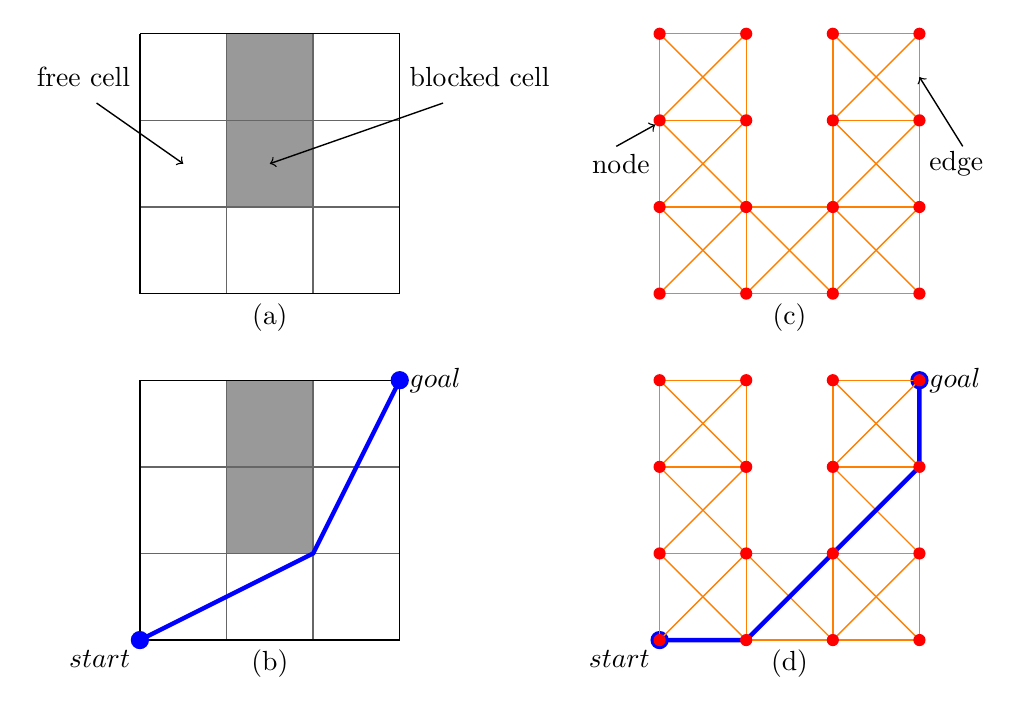
\begin{tikzpicture}[scale=1.1,line width=0.5pt]
    
      \filldraw[color=black!60,fill=black!40] (1,5) rectangle (2,7); 
      \draw[color=black!60] (0,4) grid (3,7);
      \draw[black] (0,4) -- (3,4);
      \draw[black] (0,4) -- (0,7);
      \draw[black] (3,7) -- (3,4);
      \draw[black] (3,7) -- (0,7);
      
      \node[left] at (0,6.5) {free cell};
      \draw[->] (-0.5,6.2) -- (0.5,5.5);
      \node[right] at (3,6.5) {blocked cell};
      \draw[->] (3.5,6.2) -- (1.5,5.5);

      \filldraw[color=black!60,fill=black!40] (1,1) rectangle (2,3); 
      \draw[color=black!60] (0,0) grid (3,3);
      \draw[blue, ultra thick] (0,0) -- (2,1) -- (3,3); 
      
      \draw[black] (0,0) -- (3,0);
      \draw[black] (0,0) -- (0,3);
      \draw[black] (3,3) -- (3,0);
      \draw[black] (3,3) -- (0,3);
      
      \node[right] at (3,3) {$goal$};
      \fill[blue] (3,3) circle (3pt);
      \node[below left] at (0,0) {$start$};
      \fill[blue] (0,0) circle (3pt);
     
      \fill[blue] (9,3) circle (3pt);
      \fill[blue] (6,0) circle (3pt);
     \draw[orange] (6,4) grid (9,7);
     
     \foreach \x in {6,7,8} {
        \foreach \y in {4,5,6} {
          \pgfmathparse{int(\x + 1)};
          \let\xa\pgfmathresult;
          \pgfmathparse{int(\y + 1)};
          \let\ya\pgfmathresult;
          \draw[orange] (\x,\y) -- (\xa,\ya);
        }
      }
  
      \foreach \x in {6,7,8} {
        \foreach \y in {5,6,7} {
          \pgfmathparse{int(\x + 1)};
          \let\xa\pgfmathresult;
          \pgfmathparse{int(\y - 1)};
          \let\ya\pgfmathresult;
          \draw[orange] (\x,\y) -- (\xa,\ya);
        }
      }
      
       \filldraw[color=orange,fill=white] (7,5) rectangle (8,7);
      \draw[white, ultra thick] (7,6) -- (8,6);
      \draw[white, ultra thick] (7,7) -- (8,7);

      \foreach \x in {6,7,8,9} {
        \foreach \y in {4,5,6,7} {
          \fill[red] (\x,\y) circle (2pt);
        }
      }
      
      \node[left] at (6,5.5) {node};
      \draw[->] (5.5,5.7) -- (5.95,5.95);
      \node[right] at (9,5.5) {edge};
      \draw[->] (9.5,5.7) -- (9,6.5);
    
      \draw[orange] (6,0) grid (9,3);
  
      \foreach \x in {6,7,8} {
        \foreach \y in {0,1,2} {
          \pgfmathparse{int(\x + 1)};
          \let\xa\pgfmathresult;
          \pgfmathparse{int(\y + 1)};
          \let\ya\pgfmathresult;
          \draw[orange] (\x,\y) -- (\xa,\ya);
        }
      }
  
      \foreach \x in {6,7,8} {
        \foreach \y in {1,2,3} {
          \pgfmathparse{int(\x + 1)};
          \let\xa\pgfmathresult;
          \pgfmathparse{int(\y - 1)};
          \let\ya\pgfmathresult;
          \draw[orange] (\x,\y) -- (\xa,\ya);
        }
      }

      \node[right] at (9,3) {$goal$};
      \node[below left] at (6,0) {$start$};

      \draw[blue, ultra thick] (6,0) -- (7,0) -- (9,2) -- (9,3);
      
      \filldraw[color=orange,fill=white] (7,1) rectangle (8,3);
      \draw[white, ultra thick] (7,2) -- (8,2);
      \draw[white, ultra thick] (7,3) -- (8,3);

      \foreach \x in {6,7,8,9} {
        \foreach \y in {0,1,2,3} {
          \fill[red] (\x,\y) circle (2pt);
        }
      }
      
      \node[below] at (1.5,0) {(b)};
      \node[below] at (1.5,4) {(a)};
      \node[below] at (7.5,0) {(d)};
      \node[below] at (7.5,4) {(c)};
    \end{tikzpicture}
  \caption[Shortest paths through maps and graphs]{Shortest path through a map vs. shortest path through the graph representing the map}
 \label{fig:fart}
\end{figure}

\noindent
The structure of this graph is based on the grid structure of the map. If a different graph representation was chosen then a shorter path could have been achieved, but in general such a graph would require many more nodes and edges which would cause exponentially increasing memory requirements and search space size. This dissertation will investigate various algorithms that aim to find a near-optimal path through a map while using space-efficient grid-based graph like that shown in figure 1.1(c).\\

\section{Related work}

Applying a post-processing step to smoothe paths returned by {\em A*} has been a technique that has been used since the earliest video games\cite{Thorpe84}, but most of the research into more advanced any-angle pathfinding algorithms have taken place in the last half decade. \\

\noindent
Ferguson and Stentz's paper on {\em Field D*}\cite{FergusonStentz06} in 2006 was followed by a significant contribution to the field by Nash and Koenig et al., who published papers on {\em Theta*}\cite{Daniel10} and {\em Lazy Theta*}\cite{Nash10} in 2010. In 2011, Yap's paper on {\em Block A*}\cite{Yap11} introduced the concept of pre-calculating solutions to sub-maps to speed up execution.\\

\noindent
Studies such as Nash and Koneig's article in {\em Artificial Intelligence Magazine}\cite{Nash11} have been conducted that compare a selection of these any-angle pathfinding algorithms, though the only established authority that utilises empirical data on {\em Block A*} is Yap's own work\cite{Yap11}, which compares only {\em A*}, {\em Theta*} and {\em Block A*}.

\section {Project goals}

\todo{Therefore, in this project I am aiming to reconcile the gaps in the literature by...?}

\noindent
The goals of this project are to:

\begin{itemize}
\item create an algorithm simulation environment that enables intuitive and informative comparison of the performance of the most prominent any-angle path-finding algorithms;
\item use statistical analysis to present conclusions on the suitability of these algorithms to different path-finding situations.
\end {itemize}

\cleardoublepage


\chapter{Preparation} 

\section{Introduction to any-angle pathfinding}

This section formally introduces the concept of maps and describes how graphs are created from maps. It then defines the any-angle path-finding problem.


\subsection{Map}

A map $M$ of size $N^{2}$ is a square region in two-dimensional space $[0,N]^{2} \subseteq \mathbb{R}^{2}$, where $N \in\mathbb{Z}$ and $N > 0$. A location on the map can be specified with a coordinate $(x,y) \in \mathbb{R}^{2}$, where $0 \leq x,y \leq N$.\\

\noindent
The map is logically divided into a grid of $N^{2}$ cells of size $1 \times 1$, where the cell identified by the coordinate $(i,j) \in M$ includes all locations $(x,y) \in \mathbb{R}^{2}$ where $i \leq x \leq i+1$ and $j \leq y \leq j+1$, and each cell is either `free' or `blocked'.\\

\noindent A map $M$ can be represented by a square boolean array $A_{M}$, where element $A_{M}[i][j]$ represents the cell in $M$ with coordinate $(i,j)$ --- $A_{M}[i][j] = 0$ denotes that $(i,j)$ is a free cell, whereas $A_{M}[i][j] = 1$ denotes that $(i,j)$ is a blocked cell

\begin{figure}[h]
  \begin{subfigure}{.5\textwidth}
    \centering
    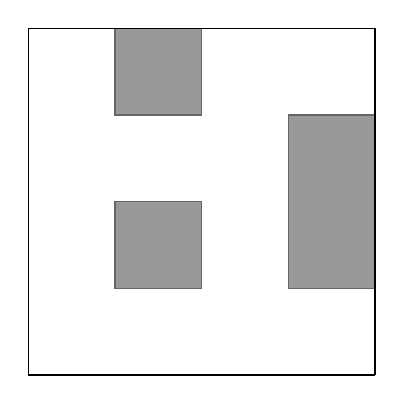
\begin{tikzpicture}[scale=1.1,line width=0.5pt]
      
      \filldraw[color=black!60,fill=black!40] (1,1) rectangle (2,2); 
      \filldraw[color=black!60,fill=black!40] (1,3) rectangle (2,4); 
      \filldraw[color=black!60,fill=black!40] (3,1) rectangle (4,3); 
      %\draw[color=black!60] (0,0) grid (4,4);
      
      \draw[black] (0,0) -- (4,0);
      \draw[black] (0,0) -- (0,4);
      \draw[black] (4,4) -- (4,0);
      \draw[black] (4,4) -- (0,4);
     
    \end{tikzpicture}
    \caption[Map]{Map $M$}
    %\label{fig:sfig1}
  \end{subfigure}
  %
  \begin{subfigure}{.5\textwidth}
    \centering
    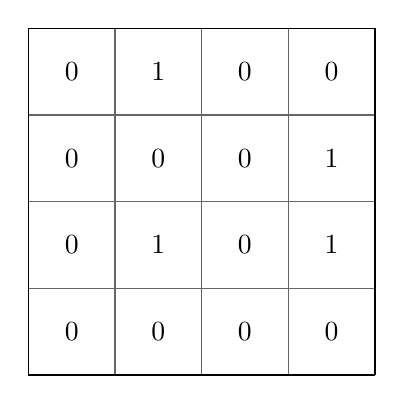
\begin{tikzpicture}[scale=1.1,line width=0.5pt]
      
      \draw[color=black!60] (0,0) grid (4,4);
      
      \draw[black] (0,0) -- (4,0);
      \draw[black] (0,0) -- (0,4);
      \draw[black] (4,4) -- (4,0);
      \draw[black] (4,4) -- (0,4);
      
      \node at (0.5,3.5){0}; \node at (1.5,3.5){1}; \node at (2.5,3.5){0};\node at (3.5,3.5){0};
      \node at (0.5,2.5){0}; \node at (1.5,2.5){0}; \node at (2.5,2.5){0}; \node at (3.5,2.5){1};
      \node at (0.5,1.5){0}; \node at (1.5,1.5){1}; \node at (2.5,1.5){0};\node at (3.5,1.5){1};
      \node at (0.5,0.5){0}; \node at (1.5,0.5){0}; \node at (2.5,0.5){0}; \node at (3.5,0.5){0};

    \end{tikzpicture}
    \caption{Array $A_{M}$ of map $M$}
    %\label{fig:sfi2}
  \end{subfigure}
  \caption{A map of size $4^{2}$}
  %\label{fig:fig}
\end{figure}

\begin{description}
\item{\bfseries Valid location}\\
The agent is modelled as a dimensionless point, as is the convention\cite{Daniel10} \todo{is this the correct way to reference it?} in any-angle pathfinding research.\footnote{It is possible to ensure that such paths are never taken by adding extra checks in the graph creation and line of sight algorithms, but this would distract from the core investigation and be an unnecessary deviation from the accepted standard.} Therefore, a valid location is defined as any location $(x,y) \in M$ that lies in or on the boundary of a free cell.
\end{description}

\begin{description}
\item{\bfseries Line of sight}\\
A line of sight exists between two locations $(x_{0},y_{0})$ and $(x_{1},y_{1})$ on a map if all locations that lie on the straight line drawn between $(x_{0},y_{0})$ and $(x_{1},y_{1})$ are valid --- that is to say, for all $t \in \mathbb{R}$ where $0 \leq t \leq 1$: $(x_{0} + t(x_{1}-x_{0}),y_{0} + t(y_{1}-y_{0}))$ is a valid location.
\end{description}

\begin{description}
\item{\bfseries Path through a map}\\
A path  $P_{M} = ((x_{0},y_{0}), (x_{1},y_{1}), \ldots, (x_{n},y_{n}))$ through map $M$ is an ordered list of coordinates $(x,y) \in \mathbb{R}^{2}$ where $0 \leq x,y \leq N$, $x_{0}=(x_{start},y_{start})$ and $x_{n}=(x_{goal},y_{goal})$. A path is valid if there exists a line of sight between every pair of coordinates $(x_{i},y_{i})$ and $(x_{i+1},y_{i+1})$.\\

\noindent
It should be noted that since the agent is modelled as a dimensionless point, the path through the map shown in Figure 2.2, which features a `diagonal blockage', is a valid path.\\

\end{description}

\begin{figure}[h]
    \centering
    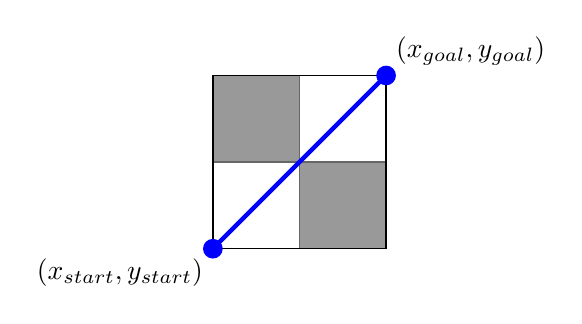
\begin{tikzpicture}[scale=1.1,line width=0.5pt]
    
      \draw[black!60] (0,0) grid (2,2);
      \filldraw[color=black!60,fill=black!40] (0,1) rectangle (1,2); 
      \filldraw[color=black!60,fill=black!40] (1,0) rectangle (2,1); 
      \draw (0,0) -- (2,0);
      \draw (0,0) -- (0,2);
      \draw (2,2) -- (2,0);
      \draw (2,2) -- (0,2);
      \node[below left] at (0,0) {$(x_{start},y_{start})$};
      \node[above right] at (2,2) {$(x_{goal},y_{goal})$};
      \filldraw[blue] (0,0) circle (3pt);
      \filldraw[blue] (2,2) circle (3pt);
      \draw[blue, ultra thick] (0,0) -- (2,2);
      
          
    \end{tikzpicture}
  \caption{A valid path for an agent modelled as a point}
  %\label{fig:fig}
\end{figure}


\subsection{Lattice}

A lattice $L_{N}$ is a graph of $N^{2}$ nodes, where $N \in\mathbb{Z}$ and $N > 0$. 

\begin{description}
\item{\bfseries Octile lattice $L_{N,O}$}\\The nodes are arranged in a square grid, and each node is connected with an edge to the closest node, if any exists, at a bearing of any integer multiple of $\frac{\pi}{4}$ radians.

\item{\bfseries Full lattice $L_{N,F}$}\\The nodes are arranged in a square grid, and each node is connected with an edge to every other node in the lattice.
\end{description}

\begin{figure}[h]
  \begin{subfigure}{.5\textwidth}
    \centering
    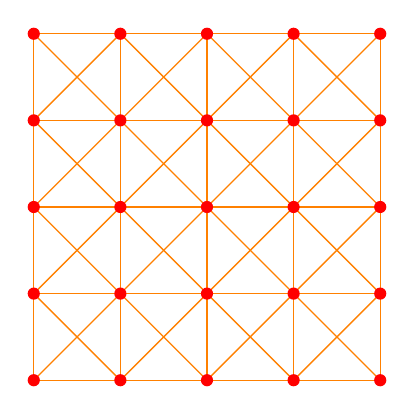
\begin{tikzpicture}[scale=1.1,line width=0.5pt]
      
      \draw[orange] (0,0) grid (4,4);
  
      \foreach \x in {0,1,2,3} {
        \foreach \y in {0,1,2,3} {
          \pgfmathparse{int(\x + 1)};
          \let\xa\pgfmathresult;
          \pgfmathparse{int(\y + 1)};
          \let\ya\pgfmathresult;
          \draw[orange] (\x,\y) -- (\xa,\ya);
        }
      }
  
      \foreach \x in {0,1,2,3} {
        \foreach \y in {1,2,3,4} {
          \pgfmathparse{int(\x + 1)};
          \let\xa\pgfmathresult;
          \pgfmathparse{int(\y - 1)};
          \let\ya\pgfmathresult;
          \draw[orange] (\x,\y) -- (\xa,\ya);
        }
      }
      
      \foreach \x in {0,1,2,3,4} {
        \foreach \y in {0,1,2,3,4} {
          \fill[red] (\x,\y) circle (2pt);
        }
      }
     
    \end{tikzpicture}
    \caption[Map]{Octile lattice $L_{N,O}$}
    %\label{fig:sfig1}
  \end{subfigure}
  %
  \begin{subfigure}{.5\textwidth}
    \centering
    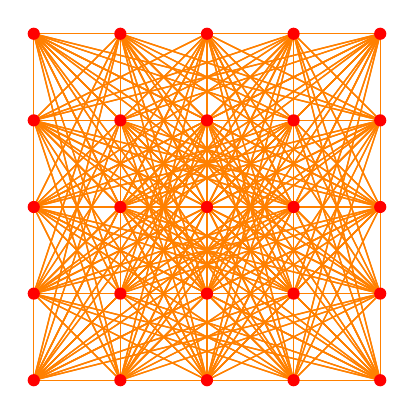
\begin{tikzpicture}[scale=1.1,line width=0.5pt]
      
      \draw[orange] (0,0) grid (4,4);
      
       \foreach \x in {0,1,2,3,4} {
        \foreach \y in {0,1,2,3,4} {
          \foreach \a in {0,1,2,3,4} {
            \foreach \b in {0,1,2,3,4} {
              \draw[orange] (\x,\y) -- (\a,\b);
            }
          }
        }
      }
      
            \foreach \x in {0,1,2,3,4} {
        \foreach \y in {0,1,2,3,4} {
          \fill[red] (\x,\y) circle (2pt);
        }
      }

    \end{tikzpicture}
    \caption{Full lattice $L_{N,F}$}
    %\label{fig:sfi2}
  \end{subfigure}
  \caption{Octile lattice and full lattice of size $4^{2}$}
  %\label{fig:fig}
\end{figure}

\subsection{Graph}

A graph $G_{M}=(V,E)$ is a discrete representation of a map $M$. Each node $n \in V$ represents a valid location $(a,b) \in M$, where $0 \leq a,b \leq N$. An agent can travel directly between the locations represented by two nodes $n$ and $n'$ if they are connected by an edge $e=(n,n') \in E$, and are thus called `neighbours'. The weight $(n,n').weight$ is the Euclidean distance an agent would traverse by travelling between the locations represented by the nodes $n$ and $n'$.\\
\begin{description}
\item{\bfseries Path through a graph}\\
A path $P_{G} = (n_{0}, n_{1}, \ldots, n_{n-1}, n_{n})$ through graph $G_{M}=(V,E)$ is a list of nodes $n \in V$, where $n_{0}=n_{start}$ and $n_{n}=n_{goal}$. A path is valid if for each pair of nodes $n_{i}$ and $n_{i+1}$ there exists an edge $(n_{i},n_{i+1}) \in E$.
\end{description}

\noindent
{\bfseries Discretisation}\\
\noindent
Discretisation is the process of creating a graph $G_{M}=(V,E)$ that represents a map $M$. The processes can be visualised as refining a lattice by removing edges and nodes from the lattice until the desired graph remains --- a node $n$ is removed if the map indicates that $n$ represents an invalid location, and an edge $(n,n')$ is removed if there is no line of sight on the map between the locations represented by $n$ and $n'$. If a grid-based graph is desired, an octile lattice is used, whereas if a visibility graph is desired, a full lattice is used.\\ 

\noindent
A more formal description of this process is now provided:

\begin{description}
\item{\bfseries Grid-based graph: $f_{G}(L_{O},M) \rightarrow G_{M,G}$}\\
An octile lattice $L_{N,O}$ is laid over $M$ such that each node in $L_{N,O}$ lies directly on top of a coordinate $(x,y)$ in $M$, where $(x,y) \in \mathbb{Z}^{2}$. If none of the (up to) four cells surrounding a node\footnote{In a map $M$ of size $N^{2}$, the four cells surrounding a node that represents coordinate $(a,b) \in M$ are the cells $(a,b)$, $(a,b-1)$, $(a-1,b-1)$ and $(a-1,b)$ if they exist, where $0 \leq a,b \leq N$.} are free then that node is removed, along with all edges that are connected to it. Additionally, if a cell is blocked, diagonal edges that cross that cell are removed, along with any horizontal or vertical edges that lie beneath the blocked cell and are also on the boundary of the lattice.

\item{\bfseries Visibility graph: $f_{V}(L_{O},M) \rightarrow G_{M,V}$}\\
A full lattice $L_{N,O}$ is laid over $M$ such that each node in $L_{N,O}$ lies directly on top of a coordinate $(x,y)$ in $M$, where $x,y \in \mathbb{Z}^{2}$. Unless {\em either} exactly three of the (up to) four cells surrounding a node are free {\em or} the node is $n_{start}$ or $n_{goal}$ then that node is removed, along with all edges that are connected to it. In addition each edge $(n,n') \in E$ is removed if there is no line of sight between the locations that $n$ and $n'$ represent.

\end{description}

\begin{figure}[h]
  \begin{subfigure}{.5\textwidth}
    \centering
    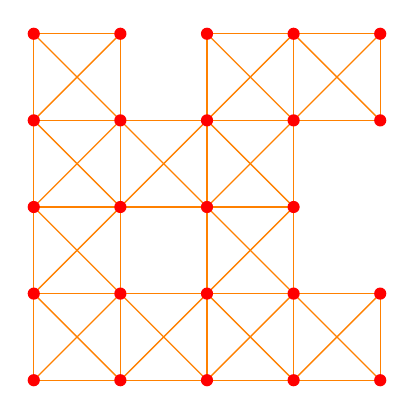
\begin{tikzpicture}[scale=1.1,line width=0.5pt]
      
      \draw[orange] (0,0) grid (4,4);
  
      \foreach \x in {0,1,2,3} {
        \foreach \y in {0,1,2,3} {
          \pgfmathparse{int(\x + 1)};
          \let\xa\pgfmathresult;
          \pgfmathparse{int(\y + 1)};
          \let\ya\pgfmathresult;
          \draw[orange] (\x,\y) -- (\xa,\ya);
        }
      }
  
      \foreach \x in {0,1,2,3} {
        \foreach \y in {1,2,3,4} {
          \pgfmathparse{int(\x + 1)};
          \let\xa\pgfmathresult;
          \pgfmathparse{int(\y - 1)};
          \let\ya\pgfmathresult;
          \draw[orange] (\x,\y) -- (\xa,\ya);
        }
      }
      
      \filldraw[color=orange,fill=white] (1,1) rectangle (2,2);
      \filldraw[color=orange,fill=white] (1,3) rectangle (2,4);
      \draw[white, ultra thick] (1,4) -- (2,4);
      \filldraw[color=orange,fill=white] (3,1) rectangle (4,3);
      \draw[white, ultra thick] (4,1) -- (4,3);
      
      \foreach \x in {0,1,2,3} {
        \foreach \y in {0,1,2,3,4} {
          \fill[red] (\x,\y) circle (2pt);
        }
      }
      \fill[red] (4,0) circle (2pt);
      \fill[red] (4,1) circle (2pt);
      \fill[red] (4,3) circle (2pt);
      \fill[red] (4,4) circle (2pt);
     
    \end{tikzpicture}
    \caption[Map]{Grid-based graph $G_{M,G}$}
    %\label{fig:sfig1}
  \end{subfigure}
  %
  \begin{subfigure}{.5\textwidth}
    \centering
    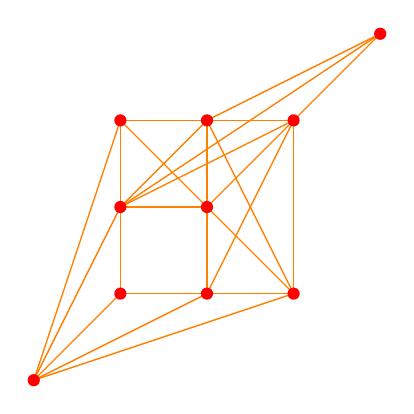
\begin{tikzpicture}[scale=1.1,line width=0.5pt]

     \draw[orange] (0,0) -- (1,1);
     \draw[orange] (0,0) -- (1,2);
     \draw[orange] (0,0) -- (1,3);
     \draw[orange] (0,0) -- (2,1);
     \draw[orange] (0,0) -- (3,1);
     
     \draw[orange] (1,1) -- (1,3);
     \draw[orange] (1,1) -- (3,1);
     
     \draw[orange] (1,2) -- (2,2);
     \draw[orange] (1,2) -- (2,3);
     \draw[orange] (1,2) -- (3,3);
     \draw[orange] (1,2) -- (4,4);
     
     \draw[orange] (1,3) -- (3,3);
     \draw[orange] (1,3) -- (3,1);
     
     \draw[orange] (2,1) -- (2,3);
     \draw[orange] (2,1) -- (3,3);
     
     \draw[orange] (2,2) -- (4,4);
     
     \draw[orange] (3,1) -- (3,3);
     \draw[orange] (3,1) -- (2,3);
     
     \draw[orange] (2,3) -- (4,4);
     
     \fill[red] (0,0) circle (2pt);
     \fill[red] (1,1) circle (2pt);
     \fill[red] (1,2) circle (2pt);
     \fill[red] (1,3) circle (2pt);
     \fill[red] (2,1) circle (2pt);
     \fill[red] (2,2) circle (2pt);
     \fill[red] (2,3) circle (2pt);
     \fill[red] (3,1) circle (2pt);
     \fill[red] (3,3) circle (2pt);
     \fill[red] (4,4) circle (2pt);
     

    \end{tikzpicture}
    \caption{Visibility graph $G_{M,V}$}
    %\label{fig:sfi2}
  \end{subfigure}
  \caption[Graph representations of map $M$]{Graph representations of map $M$, where $n_{start} = (0,0)$ and $n_{goal} = (4,4)$}
  %\label{fig:fig}
\end{figure}

\newpage
\subsection{The any-angle pathfinding problem}

The problem is to compute optimal or near-optimal paths, if they exist, through maps.\\

\noindent
\todo{Need to sort out wording here}
An optimal path $P^{*}_{M}$ through map $M$ is a path $P_{M}$ has a path length that is no longer than the path length of any other paths through $M$. If there exists more than one path with this shortest path length, the optimal paths are the paths with the shortest path length and the smallest path angle-sum, where:

\begin{description}
\item{\bfseries Path length}\\
The length of path $P_{M}$ is the sum of the Euclidean distances between each pair of coordinates $(x_{i},y_{i})$ and $(x_{i+1},y_{i+1})$ in $P_{M}$.
\item{\bfseries Path angle-sum}\\
The angle-sum of path $P_{M}$ is the sum of the smallest angle between each pair of path segments $(x_{i},y_{i})$ to $(x_{i+1},y_{i+1})$ and $(x_{i+1},y_{i+1})$ to $(x_{i+2},y_{i+2})$ in $P_{M}$.
\end{description}

\subsection{Solving the any-angle pathfinding problem}

\noindent
An optimal or near-optimal path through map $M$ is obtained by applying a pathfinding algorithm\footnote{{\em Block A*} operates in a different way, and will be dealt with separately.} to a graph $G_{M}$. The path $P_{G} = (n_{0},n_{1},...,n_{n})$  returned by the pathfinding algorithm corresponds to the path $P_{M} = (x_{0},x_{1},...,x_{n})$, where $x_{i}$ is the location represented by $n_{i}$.

\begin{description}
\item{\bfseries Classic pathfinding algorithm}\\ 
A classic pathfinding algorithm will return the optimal\footnote{The optimal path $P^{*}_{G}$ through graph $G$ is defined analogously to the optimal path $P^{*}_{M}$ through map $M$.} path $P^{*}_{G}$ through $G_{M}$.
\item{\bfseries Any-angle pathfinding algorithm}\\
An any-angle pathfinding algorithm will return the optimal path $P^{*}_{G'}$ through $G'_{M}$, where the augmented graph $G'_{M}$ may have extra edges to $G_{M}$.
\end{description}

\noindent
The optimal path $P^{*}_{G}$ through a visibility graph $G_{M,V}$ directly corresponds to the optimal path $P^{*}_{M}$ through map $M$, whereas the optimal path through a grid-based graph $G_{M,G}$ or an augmented graph $G_{M,G'}$ may not. However, grid-based graphs are generally accepted as the preferable form of map representation for pathfinding since, for a map $M$ of size $N^{2}$, $G_{M,G}$ has {$O(N^{2})$} edges, whereas $G_{M,V}$ has {$O(N^{4})$} edges, which may be unfeasible for large or high resolution maps. Therefore, this investigation will focus predominantly on pathfinding algorithms applied to grid-based graphs.\\

\newpage
\section{Any-angle pathfinding algorithms}

\noindent
This section starts with an introduction of pathfinding over graphs. It then describes two classic pathfinding algorithms: {\em Dijktra's shortest paths}\cite{Dij59} and {\em A*}\cite{Hart68}, followed by the four any-angle pathfinding algorithms that form the core investigation in this dissertation: {\em A* with post smoothing}, {\em Theta*}, {\em Lazy Theta*} and {\em Block A*}.

\subsection{Pathfinding over graphs}

\noindent
Section 2.1.3 introduced the concept of a graph $G_{M}$ that is a representation of a map $M$. In addition to an associated coordinate, each node $n$ in $G_{M}$ has a set of parameters of which the values will change during the execution of the pathfinding algorithm. These parameters include:
\begin{itemize}
\item {\em g-value} --- the path length of the shortest path found so far from $n_{start}$ to $n$;
\item {\em parent} --- a pointer to the previous node in the shortest path found so far from $n_{start}$ to $n$.
\end{itemize}

\noindent
When the algorithm is initialised, $n.g = \infty$ and $n.parent = \bot$\footnote{Where $\bot$ denotes that the parameter value is undefined.} for all nodes.\\

\noindent
When the algorithm terminates, $n_{goal}.g$ is the path length of the shortest path, if one exists, found by the algorithm from $n_{start}$ to $n_{goal}$, and the shortest path, if one exists, can be found by recursively following the $parent$ pointers from $n_{goal}$ to $n_{start}$\footnote{The pathfinding algorithm guarantees $n_{start}.parent = \bot$.}.

\subsection {Dijkstra's shortest paths}

Most of the algorithms in this dissertation are derivatives of the {\em A*} graph traversal algorithm, which itself is a derivative of {\em Dijkstra}'s famous shortest-path algorithm.\\

\noindent
{\bf Explanation}\\
\noindent
Starting with $n_{start}$, {\em Dijkstra} processes (or `expands') nodes from $G_{M}$ until it processes $n_{goal}$, at which point it terminates. Each node is expanded at most once, since it is a provable\cite{CormenDijkstra} invariant of the algorithm that when a node $n$ is selected to be processed, $n.g$ is the length of the shortest path in the graph to $n$ from $n_{start}$ --- a set $closedSet$\footnote{The set and priority queue methods $add()$, $pop()$ and  $contains()$ are defined in the usual way.} ensures that no node is expanded twice, as this would incur unnecessary work.\\

\noindent
{\bf Iteration}\\
\noindent
On each iteration, {\em Dijkstra} selects a node $n$ to expand from $openSet$, a priority queue that stores nodes in increasing order of their {\em g-values}. For each $n_{neigh}$ of the neighbours of $n$, {\em Dijkstra} attempts to `relax' $n_{neigh}$ --- that is to say: {\em Dijkstra} tests whether the shortest path to $n_{neigh}$ that has been found so far is longer than the path to $n_{neigh}$ that goes via $n$:
\begin{equation}
n.g + (n,n_{neigh}).weight < n_{neigh}.g
\end{equation}
\noindent
and if (2.1) is true, {\em Dijkstra} updates $n_{neigh}$ so that the shortest path to it is via $n$, by: 
\begin{itemize}
\item updating the {\em g-value} of $n_{neigh}$ to $n.g + (n,n_{neigh}).weight$  
\item updating the $parent$ of $n_{neigh}$ to $n$;
\item adding $n_{neigh}$ to $openSet$ if it is not already in it.
\end{itemize}

\noindent
{\bf Termination}\\
\noindent
This process continues until $openSet$ is empty or $n_{goal}$ has been processed, at which point the algorithm terminates. If a valid path exists, {\em Dijkstra} returns $P^{*}_{G}$. Otherwise it returns $\bot$.\

\begin{algorithm}
  \SetAlgoLined\DontPrintSemicolon
  \SetKwFunction{dijkstra}{Dijkstra}\SetKwFunction{update}{Update}
  \SetKwProg{myDef}{def}{}{}
  \myDef{\dijkstra{G, $n_{start}$, $n_{goal}$}}{
  \nl $openSet \gets \bot$\;
  \nl $closedSet \gets \bot$\;
  \nl $n_{start}.g \gets 0$\;
  \nl $openSet.add(n_{start})$\;
  \nl \While{$openSet \neq \bot$} {
    \nl $n_{curr} \gets openSet.pop()$\;
    \nl $closedSet.add(n_{curr})$\;
    \nl \If{$n_{curr} = n_{goal}$} {
      \nl \KwRet{$n_{goal}$}\;
    }
    \nl \ForEach{$n_{neigh}$ of $n_{curr} $} {
      \nl \If{$closedSet.contains(n_{neigh}) = false $} {
        \nl \If{$\update(n_{neigh}) = true$} {
          \nl \If{$openSet.contains(n_{neigh}) = false $} {
            \nl $openSet.add(n_{neigh})$\;
          }
        }
      }
    }
  }
  \nl \KwRet{$\bot$}\;
}{}
  \setcounter{AlgoLine}{0}
  \myDef{\update{$n_{neigh}$}}{
    \nl \uIf{$n_{curr}.g + (n_{curr},n_{neigh}).weight < n_{neigh}.g$} {
      \nl $n_{neigh}.g = n_{curr}.g + (n_{curr},n_{neigh}).weight$\;
      \nl $n_{neigh}.parent = n_{curr}$\;
      \nl \KwRet{$true$}\;
    } \nl \Else {
      \nl \KwRet{$false$}\;
    } 
  }
  \caption{{\sc Dijkstra}}
\end{algorithm} 

\subsection {A*}

{\em A*} is based on {\em Dijkstra's shortest-paths} algorithm, but uses a heuristic $h$ to reduce the number of nodes expanded.\\

\noindent
In addition to a {\em g-value} and a {\em parent}, each node also has a\todo{Arbitrary choice between node having h-value or f-value?}:
\begin{itemize}
\item {\em h-value} --- Euclidean distance between {$n$} and {$n_{goal}$}: a cheaply computable monotonic estimate\footnote{The monotonicity of Euclidean distance as a heuristic ensures that {\em A*}, like {\em Dijkstra}, is complete (if a path exists, it finds it) and optimal (if a path is found, it is a shortest distance path)} of the actual shortest path length between $n$ and $n_{goal}$.
\end{itemize}

\noindent
While {\em Dijkstra} preferentially expands nodes with low {\em g-value}s, {\em A*} preferentially expands nodes with low {\em f-score}s, where a node $n$'s {\em f-score} is the algorithms current estimate of the shortest path from $n_{start}$ to $n_{goal}$ that goes via $n$ --- that is to say:
\begin{equation}
n.f = n.g + n.h
\end{equation}

\noindent
The pseudocode for {\em A*} differs only from {\em Dijkstra} in the {\tt update} subroutine, where the {\em h-score} must also be set.

\begin{algorithm}
  \SetAlgoLined\DontPrintSemicolon
  \SetKwFunction{update}{Update}
  \SetKwProg{myDef}{def}{}{}
  \myDef{\update{$n_{neigh}$}}{
    \nl \uIf{$n_{curr}.g + (n_{curr},n_{neigh}).weight < n_{neigh}.g$} {
      \nl $n_{neigh}.g \gets n_{curr}.g + euclidean(n_{curr},n_{neigh})$\;
      \nl $n_{neigh}.h \gets euclidean(n_{neigh},n_{goal})$\;
      \nl $n_{neigh}.parent = n_{curr}$\;
      \nl \KwRet{$true$}\;
    } \nl \Else {
      \nl \KwRet{$false$}\;
    } 
  }
  \caption{{\tt Update} from {\sc A*}}
\end{algorithm} 

\subsection {A* with post-smoothing}

A post-processing step is run on the path $P_{G} = (n_{start}, n_{1}, \ldots, n_{n-1}, n_{goal})$ returned by {\em A*}, which attempts to reduce the path distance by changing the {\em parent} pointer of some of the elements of $P_{G}$ --- this has the effect of adding new edges to the graph $G$ to create a new graph $G'$.\\

\noindent
{\bf Iteration}\\
\noindent
On each iteration, the algorithm considers a node $n_{curr}$. Starting with $n_{curr} = n_{goal}$ a line of sight test is performed from the coordinate associated with $n_{curr}$ to the coordinate associated with $n_{curr}.parent.parent$. If a line of sight exists, $n_{curr}.parent$ is set to $n_{curr}.parent.parent$ --- this has the effect of adding an edge $(n_{curr},n_{curr}.parent.parent)$ to $G$. This process is repeated on $n_{curr}$ until a line of sight test fails, at which point $n_{curr}$ is set to $n_{curr}.parent.parent$\footnote{Note: $n_{curr}.parent.parent$ is the node on which the line of sight test failed.}, and the next iteration commences. \\

\noindent
{\bf Termination}\\
\noindent
When $n = n_{start}$, the algorithm terminates.\\

\begin{figure}[h]
  \begin{subfigure}{.3\textwidth}
    \centering
    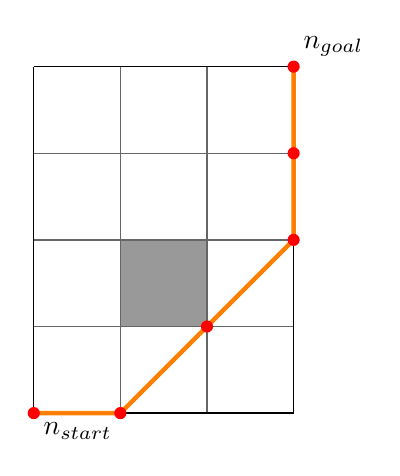
\begin{tikzpicture}[scale=1.1,line width=0.5pt]
    
      \draw[color=black!60] (0,0) grid (3,4);
    
      \node[below right] at (0,0) {$n_{start}$};
      \node[above right] at (3,4) {$n_{goal}$};

      \filldraw[color=black!60,fill=black!40] (1,1) rectangle (2,2); 
      \draw (0,0) -- (0,4);
      \draw (0,0) -- (3,0);
      \draw (3,4) -- (0,4);
      \draw (3,4) -- (3,0);
    
      \draw[orange, ultra thick] (0,0) -- (1,0) -- (3,2) -- (3,4);
      \fill[red] (0,0) circle (2pt);
      \fill[red] (1,0) circle (2pt);
      \fill[red] (2,1) circle (2pt);
      \fill[red] (3,2) circle (2pt);
      \fill[red] (3,3) circle (2pt);
      \fill[red] (3,4) circle (2pt);

    \end{tikzpicture}
    \caption{Original path}
    %\label{fig:sfi2}
  \end{subfigure}
  \begin{subfigure}{.3\textwidth}
    \centering
    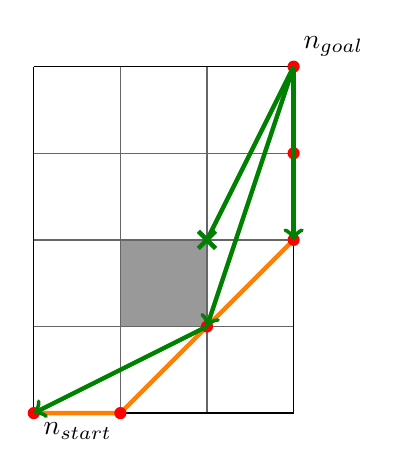
\begin{tikzpicture}[scale=1.1,line width=0.5pt]
    
      \draw[color=black!60] (0,0) grid (3,4);
    
      \node[below right] at (0,0) {$n_{start}$};
      \node[above right] at (3,4) {$n_{goal}$};

      \filldraw[color=black!60,fill=black!40] (1,1) rectangle (2,2); 
      \draw (0,0) -- (0,4);
      \draw (0,0) -- (3,0);
      \draw (3,4) -- (0,4);
      \draw (3,4) -- (3,0);
      
      \draw[orange, ultra thick] (0,0) -- (1,0) -- (3,2) -- (3,4);
      \fill[red] (0,0) circle (2pt);
      \fill[red] (1,0) circle (2pt);
      \fill[red] (2,1) circle (2pt);
      \fill[red] (3,2) circle (2pt);
      \fill[red] (3,3) circle (2pt);
      \fill[red] (3,4) circle (2pt);
      
      \draw[green!50!black, ultra thick,->] (3,4) -- (3,2);
      \draw[green!50!black, ultra thick,->] (3,4) -- (2,1);
      \draw[green!50!black, ultra thick] (3,4) -- (2,2);
      %\draw[red!20,thick,->] (2,2) -- (1,0);
      \draw[green!50!black,ultra thick] (1.9,2.1) -- (2.1,1.9);
      \draw[green!50!black,ultra thick] (1.9,1.9) -- (2.1,2.1);
      \draw[green!50!black, ultra thick, ->] (2,1) -- (0,0);


    \end{tikzpicture}
    \caption{Line of sight tests} \label{fig:astarsmoothed}
  \end{subfigure}
  %
  \begin{subfigure}{.3\textwidth}
    \centering
    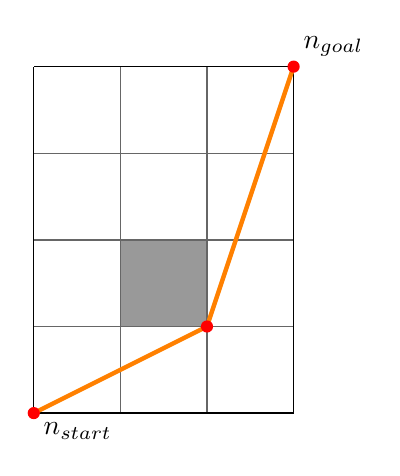
\begin{tikzpicture}[scale=1.1,line width=0.5pt]
    
      \draw[color=black!60] (0,0) grid (3,4);
    
      \node[below right] at (0,0) {$n_{start}$};
      \node[above right] at (3,4) {$n_{goal}$};

      \filldraw[color=black!60,fill=black!40] (1,1) rectangle (2,2); 
      \draw (0,0) -- (0,4);
      \draw (0,0) -- (3,0);
      \draw (3,4) -- (0,4);
      \draw (3,4) -- (3,0);
    
      \draw[orange, ultra thick] (0,0) -- (2,1) -- (3,4);
      \fill[red] (0,0) circle (2pt);
      \fill[red] (2,1) circle (2pt);
      \fill[red] (3,4) circle (2pt);

    \end{tikzpicture}
    \caption{Improved path}
    %\label{fig:sfi2}
  \end{subfigure}
  \caption{A* with post-smoothing}
  %\label{fig:fig}
\end{figure}


\begin{algorithm}
  \SetAlgoLined\DontPrintSemicolon
  \SetKwFunction{ps}{PostSmoothing}\SetKwFunction{los}{LineOfSight}
  \SetKwProg{myDef}{def}{}{}
  \myDef{\ps{$n_{start}, n_{goal}$}}{
    \nl $n_{curr} \gets n_{goal} $\;
    \nl $n_{next} \gets n_{goal}.parent.parent $\;
    \nl \uIf {$n_{next}  = \bot$} {
      \nl \KwRet{} \;
    }
    \nl \While{$true$} {
      \nl \While{$\los(n_{curr} ,n_{next} )$} {
        \nl $n_{curr}.parent \gets n_{next} $\;
        \nl $n_{next}  \gets n_{next} .parent$\;
        \nl \uIf{$n_{next}  = n_{start}$} {
          \nl \KwRet{} \;
        }
      }
      \nl $n_{curr}  \gets n_{next} $\;
      \nl \uIf{$n_{curr}.parent = n_{start}$} {
        \nl \KwRet{}\;
        }
      \nl $n_{next}  \gets n_{next}.parent.parent$\;
    }
  }
  \caption{{\tt PostSmoothing} from {\sc A* with post-smoothing}}
\end{algorithm} 

\subsection {Theta*}

Where {\em A* with post-smoothing} performs an explicit smoothing step after finding the basic path with {\em A*}, {\em Theta*} interleaves smoothing with exploration by attempting to re-parent each of $n_{curr}$'s neighbours $n_{neigh}$ with $n_{curr}.parent$ at the time when $n_{curr}$ is expanded\footnote{As with {\em A* with post-smoothing}, re-parenting in {\em Theta*} occurs if a line of sight exists between the coordinates represented by the two nodes in question.}.\\

\noindent
The pseudocode for {\em Theta*} differs only from {\em A*} in the {\tt update} subroutine. If a line of sight exists between the coordinates represented by $n_{neigh}$ and $n_{curr}.parent$, {\em Theta*} (notionally) creates an edge $e = (n_{neigh}, n_{curr}.parent)  \in G$ and attempts to relax $e$. If the line of sight does not exist, $e$ is removed from $G$ and {\em Theta*} mimics {\em A*} by attempting to relax the edge $(n_{neigh},n_{curr})$\footnote{As per the {\tt update} subroutine of {\em A*}.}.

\begin{algorithm}
  \SetAlgoLined\DontPrintSemicolon
  \SetKwFunction{update}{Update}\SetKwFunction{los}{LineOfSight}
  \SetKwProg{myDef}{def}{}{}
  \myDef{\update{$n_{neigh}$}}{
    \nl \uIf{$\los(n_{neigh}, n_{curr}.parent) = true$} {
      \nl \uIf{$n_{curr}.parent.g + (n_{curr}.parent,n_{neigh}).weight < n_{neigh}.g$} {
        \nl $n_{neigh}.g \gets n_{neigh}.parent.g + (n_{curr}.parent,n_{neigh}).weight$\;
        \nl $n_{neigh}.f \gets euclidean(n_{neigh},n_{goal})$\;
        \nl $n_{neigh}.parent \gets n_{curr}.parent$\;
        \nl \KwRet{$true$}\;
      } \nl \Else {
        \nl \KwRet{$false$}\;
      } 
    } \nl \Else {
      \nl \uIf{$n_{curr}.g + (n_{curr},n_{neigh}).weight < n_{neigh}.g$} {
        \nl $n_{neigh}.g \gets n_{curr}.g + (n_{curr},n_{neigh}).weight$\;
        \nl $n_{neigh}.f \gets euclidean(n_{neigh},n_{goal})$\;
        \nl $n_{neigh}.parent \gets n_{curr}$\;
        \nl \KwRet{$true$}\;
      } \nl \Else {
        \nl \KwRet{$false$}\;
      } 
    }
  }
  \caption{{\tt Update} from {\sc Theta*}}
\end{algorithm} 

\subsection {Lazy Theta*}

{\em Lazy Theta*} attempts to refine {\em Theta*} by finding similar paths despite performing fewer line of sight tests. Where {\em Theta*} performs a line of sight for every neighbour $n_{neigh}$ of every node $n_{curr}$ that is expanded, {\em Lazy Theta*} avoids unnecessary line of sight tests by only performing them for every node $n_{curr}$ that is expanded. \\

\noindent
{\bf Iteration}\\
\noindent
For each $n_{curr}$ that is expanded, {\em Lazy Theta*} assumes that a line of sight exists between $n_{curr}.parent$ and each neighbour $n_{neigh}$ of $n_{curr}$, and updates the {\em g-value} and $parent$ of each $n_{neigh}$ accordingly\footnote{{\em Lazy Theta*} performs the update part of relaxation without first performing the test in equation (2.1)}. {\em Lazy Theta*} only actually performs that line of sight test if the $n_{neigh}$ itself is ever expanded (henceforth referred to as $n_{curr}'$, for clarity), by calling {\tt Initialise} when $n_{curr}'$ is popped off $openSet$. If the line of sight doesn't in fact exist, {\tt Initialise} alters $n_{curr}'$ accordingly\footnote{See {\bfseries Algorithm 5} lines 2-4}.

\begin{algorithm}
  \SetAlgoLined\DontPrintSemicolon
  \SetKwFunction{update}{Update}\SetKwFunction{los}{LineOfSight}\SetKwFunction{init}{Initialise}
  \SetKwProg{myDef}{def}{}{}
  \myDef{\init{$n_{curr}$}}{
      \nl \uIf{$\los(n_{curr}, n_{curr}.parent) = false$} {
        \nl $newParent \gets \argmin\limits_{n' \in expandedNeigh(n_{curr})} (n'.g + (n',n_{curr}).weight)$\;
        \nl $n_{curr}.parent \gets n'$\;
        \nl $n_{curr}.g \gets n'.g + (n',n_{curr}).weight$\;
       } 
  }
  \myDef{\update{$n_{neigh}$}}{
        \tcp{assume line of sight test passes}
      \nl \uIf{$n_{curr}.parent.g + (n_{curr}.parent,n_{neigh}).weight < n_{neigh}.g$} {
        \nl $n_{neigh}.g \gets n_{neigh}.parent.g + (n_{curr}.parent,n_{neigh}).weight$\;
        \nl $n_{neigh}.f \gets euclidean(n_{neigh},n_{goal})$\;
        \nl $n_{neigh}.parent \gets n_{curr}.parent$\;
        \nl \KwRet{$true$}\;
      } \nl \Else {
        \nl \KwRet{$false$}\;
      } 
  }
  \caption{{\tt Initialise} and {\tt Update} from {\sc Lazy Theta*}}
\end{algorithm} 

\noindent
It should be noted that when run on a given map, {\em Lazy Theta*} does not necessarily return the same path as {\em Theta*}.

\subsection {Block A*}

\noindent
{\em Block A*} is the most complex algorithm in this dissertation. It was published in 2011, and is at the very cutting edge of any-angle path-finding algorithmic research. This dissertation attempts a novel explanation of {\em Block A*} that draws closer parallels with the graph-based explanations provided in the previous sections for {\em Dijkstra} and {\em A*}.\\

\noindent
{\bfseries Overview}\\
\noindent
{\em Block A*} divides a map $M$ into logical blocks and then finds an optimal or near-optimal path by proceeding through $M$ in a block by block fashion, as opposed to node by node like the other algorithms studied in this dissertation. This gives {\em Block A*} the potential for fast evaluation. {\em Block A*} uses the concept of a {\em Local Distance Database} to provide information about shortest paths {\em through} blocks without having to explicitly calculate them.\\

\noindent
{\bfseries Blocks}\\
\noindent
Where all of the previously introduced algorithms operate on a simple graph structure, {\em Block A*} operates on a structure based on blocks. A block $B_{i,j}$ of size $N_{B}^{2}$, identified by the coordinate $(i,j) \in \mathbb{Z}^{2}$, is a graph that represents the subsection of a map $M$ containing all locations $(x,y) \in \mathbb{R}^{2}$, where $i \leq x \leq i+N_{B}$ and $j \leq y \leq j+N_{B}$.\\

\noindent
For each block $B_{i,j} = (V_{i,j},E_{i,j})$, $n \in V_{i,j}$ represents a location $(a,b) \in \mathbb{Z}^{2}$ in $M$ where $(a,b)$ lies on the boundary of the $B_{i,j}$ --- that is to say, where $a=i$ or $a=i+N_{B}$, and $b=j$ or $b=j+N_{B}$. In addition to an associated coordinate, each node $n \in B_{i,j}$ has the parameters:
\begin{itemize}
\item {\em g-value} --- the path length of the shortest path found so far from $start$\footnote{In {\em Block A*} there is no explicit node $n_{start}$ or $n_{goal}$ --- $start$ and $goal$ are coordinates $(x,y) \in \mathbb{R}^{2}$ in $M$.} to $n$;
\item {\em h-value} --- Euclidean distance between $n$ and $goal$\footnote{Except when the block is $B_{goal}$, when the {\em h-value} is the length of the shortest path between $n$ and $goal$ --- this is discussed in the `Initialisation' step.}. 
\item {\em parent} --- the previous node in the shortest path found so far from $start$ to $n$
\end{itemize}

\noindent
Each $block$ $B_{i,j}$ maintains an unordered $openSet_{i,j} \subseteq V_{i,j}$, and a $heapValue_{i,j}$. $heapValue_{i,j}$ is the smallest {\em f-score} of the nodes in $openSet_{i,j}$\footnote{If $openSet_{i,j} = \bot$, $B_{i,j}.heapValue = \infty$.}, and is used to order blocks in $openSet_{blocks}$, a priority queue that stores blocks in increasing order of their $heapValue$s.\\

\noindent
If the locations represented by $B_{i,j}$ contain the location $start$ or $goal$ then $B_{i,j}$ is called $B_{start}$ or $B_{goal}$ respectively, and $B_{i,j}$ has an extra node $n_{start}$ or $n_{goal}$ with an edge from that node to every other node in the block. For all other blocks, called 'regular' blocks, there is an edge between every pair of nodes in $B_{i,j}$. See figure 2.7. For all edges $(n,n') \in B$, {\em $(n,n').weight$ is the length of the shortest path in map $M$ between the two locations represented by $n$ and $n'$, and $0 \leq $(n,n').weight$ \leq \infty$}. This important distinction bears clarificiation: in grid-based graphs and visibility graphs, an edge denotes that an agent can travel in a straight line between the two nodes that the edge connects, whereas an edge in a block merely denotes that an agent can travel between those two nodes {\em on some path within that block}, where the length of that path is the edge weight which may range from $0$ to $\infty$. See figure 2.7\\

\begin{figure}
    \centering
    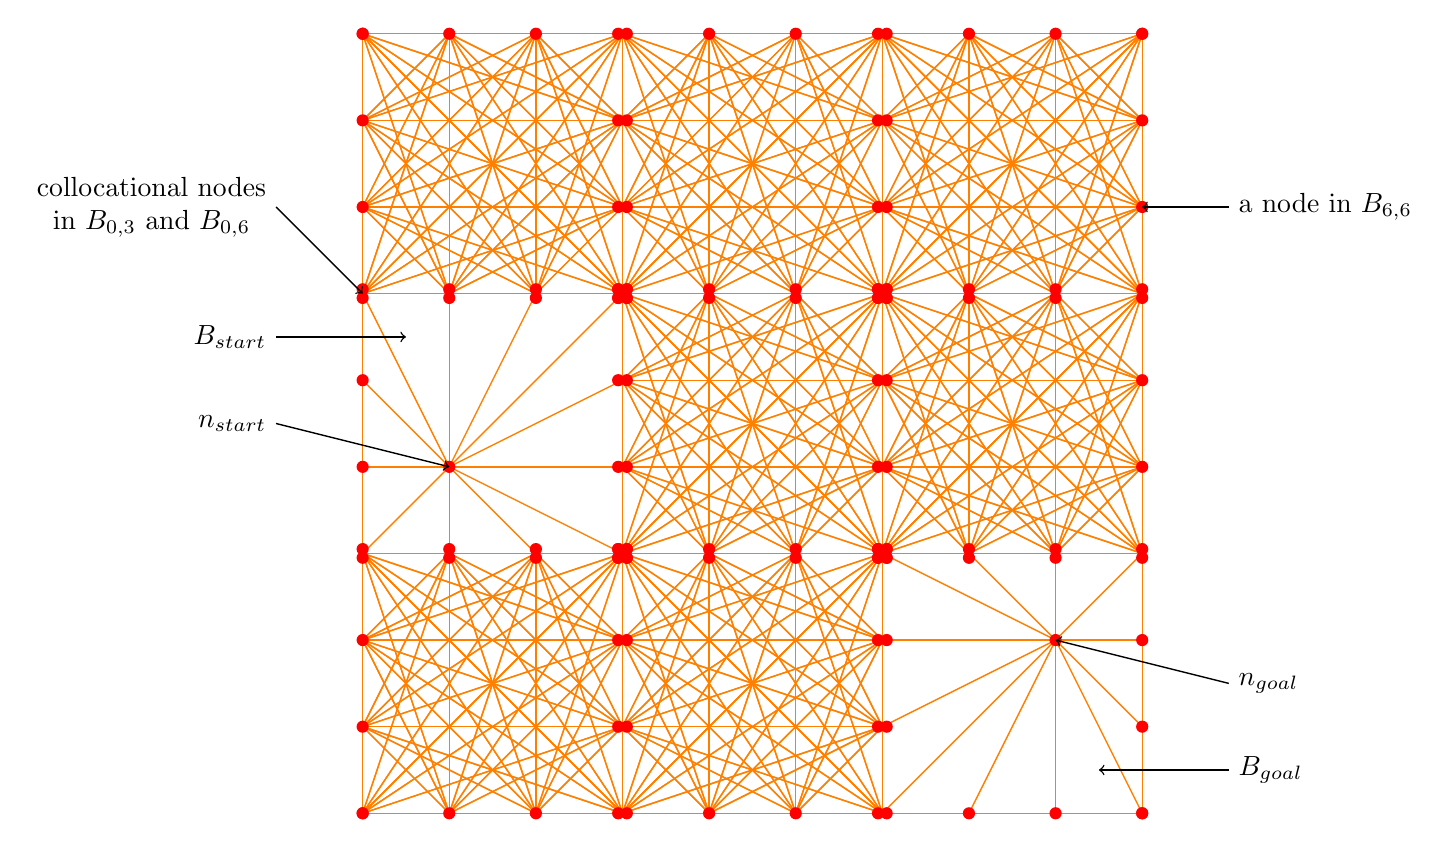
\begin{tikzpicture}[scale=1.1,line width=0.5pt]
  
      \foreach \i in {0,3,6} {
      \foreach \j in {0,3,6} {
      \foreach \x in {0,1,2,3} {
        \foreach \y in {0,3} {
          \foreach \a in {0,1,2,3} {
            \foreach \b in {0,3} {
             \pgfmathparse{int(\x + \i)};
             \let\xn\pgfmathresult;
             \pgfmathparse{int(\a + \i)};
             \let\an\pgfmathresult;
             \pgfmathparse{int(\y + \j)};
             \let\yn\pgfmathresult;
             \pgfmathparse{int(\b + \j)};
             \let\bn\pgfmathresult;
              \draw[orange] (\xn,\yn) -- (\an,\bn);
              \draw[orange] (\yn,\xn) -- (\bn,\an);
            }
          }
        }
      }
      }}
      
      \foreach \i in {0,3,6} {
      \foreach \j in {0,3,6} {
      \foreach \x in {1,2} {
        \foreach \y in {0,3} {
          \foreach \a in {1,2} {
            \foreach \b in {0,3} {
             \pgfmathparse{int(\x+\i)};
             \let\xn\pgfmathresult;
             \pgfmathparse{int(\a+\j)};
             \let\an\pgfmathresult;
             \pgfmathparse{int(\y+\j)};
             \let\yn\pgfmathresult;
             \pgfmathparse{int(\b+\i)};
             \let\bn\pgfmathresult;
              \draw[orange] (\xn,\yn) -- (\bn,\an);
              \draw[orange] (\yn,\xn) -- (\an,\bn);
            }
          }
        }
      }
      }}
      
      \filldraw[color=orange, fill=white] (0,3) rectangle (3,6);
      \filldraw[color=orange, fill=white] (6,0) rectangle (9,3);
      
      \draw[orange] (1,4) -- (0,3);
      \draw[orange] (1,4) -- (0,4);
      \draw[orange] (1,4) -- (0,5);
      \draw[orange] (1,4) -- (0,6);
      \draw[orange] (1,4) -- (3,3);
      \draw[orange] (1,4) -- (3,4);
      \draw[orange] (1,4) -- (3,5);
      \draw[orange] (1,4) -- (3,6);
      \draw[orange] (1,4) -- (1,3);
      \draw[orange] (1,4) -- (2,3);
      \draw[orange] (1,4) -- (1,6);
      \draw[orange] (1,4) -- (2,6);
      \fill[red] (1,4) circle (2pt);
      \draw[orange] (8,2) -- (6,0);
      \draw[orange] (8,2) -- (6,1);
      \draw[orange] (8,2) -- (6,2);
      \draw[orange] (8,2) -- (6,3);
      \draw[orange] (8,2) -- (9,0);
      \draw[orange] (8,2) -- (9,1);
      \draw[orange] (8,2) -- (9,2);
      \draw[orange] (8,2) -- (9,3);
      \draw[orange] (8,2) -- (7,0);
      \draw[orange] (8,2) -- (8,0);
      \draw[orange] (8,2) -- (7,3);
      \draw[orange] (8,2) -- (8,3);
      \fill[red] (8,2) circle (2pt);
      
      \foreach \x in {0,1,2,2.95,3.05,4,5,5.95,6.05,7,8,9} {
        \foreach \y in {0,9} {
              \fill[red] (\x,\y) circle (2pt);
              \fill[red] (\y,\x) circle (2pt);
        }
      }
      
      \foreach \x in {1,2,4,5,7,8} {
        \foreach \y in {3,6} {
          \pgfmathparse{(\y + 0.05)};
           \let\ya\pgfmathresult;
            \pgfmathparse{(\y - 0.05)};
           \let\yb\pgfmathresult;
              \fill[red] (\x,\ya) circle (2pt);
              \fill[red] (\x,\yb) circle (2pt);
              \fill[red] (\ya,\x) circle (2pt);
              \fill[red] (\yb,\x) circle (2pt);
        }
      }
      
       \foreach \x in {3,6} {
        \foreach \y in {3,6} {
          \pgfmathparse{(\x + 0.05)};
           \let\xa\pgfmathresult;
            \pgfmathparse{(\x - 0.05)};
           \let\xb\pgfmathresult;
           \pgfmathparse{(\y + 0.05)};
           \let\ya\pgfmathresult;
              \fill[red] (\xa,\ya) circle (2pt);
              \fill[red] (\xb,\ya) circle (2pt);
              \fill[red] (\ya,\xa) circle (2pt);
              \fill[red] (\ya,\xb) circle (2pt);
        }
      }
      
             \foreach \x in {3,6} {
        \foreach \y in {3,6} {
          \pgfmathparse{(\x + 0.05)};
           \let\xa\pgfmathresult;
            \pgfmathparse{(\x - 0.05)};
           \let\xb\pgfmathresult;
           \pgfmathparse{(\y - 0.05)};
           \let\ya\pgfmathresult;
              \fill[red] (\xa,\ya) circle (2pt);
              \fill[red] (\xb,\ya) circle (2pt);
              \fill[red] (\ya,\xa) circle (2pt);
              \fill[red] (\ya,\xb) circle (2pt);
        }
      }
      
      \node[left] at (-1,5.5) {$B_{start}$};
      \draw[->] (-1,5.5) -- (0.5,5.5);
      
      \node[left] at (-1,4.5) {$n_{start}$};
      \draw[->] (-1,4.5) -- (1,4);
      
      \node[right] at (10,1.5) {$n_{goal}$};
      \draw[->] (10,1.5) -- (8,2);
      
      \node[right] at (10,0.5) {$B_{goal}$};
      \draw[->] (10,0.5) -- (8.5,0.5);
      
      \node[right] at (10,7) {a node in $B_{6,6}$};
      \draw[->] (10,7) -- (9,7);
      
      \node[left,align=center] at (-1,7) {collocational nodes \\in $B_{0,3}$ and $B_{0,6}$};
      \draw[->] (-1,7) -- (0,6);
      
     
    \end{tikzpicture}
    \caption[Set of blocks]{Logical view of a map of size $9^{2}$ as a set of 9 blocks of size $3^{2}$}
  %\label{fig:fig}
\end{figure}


\begin{figure}
    \centering
    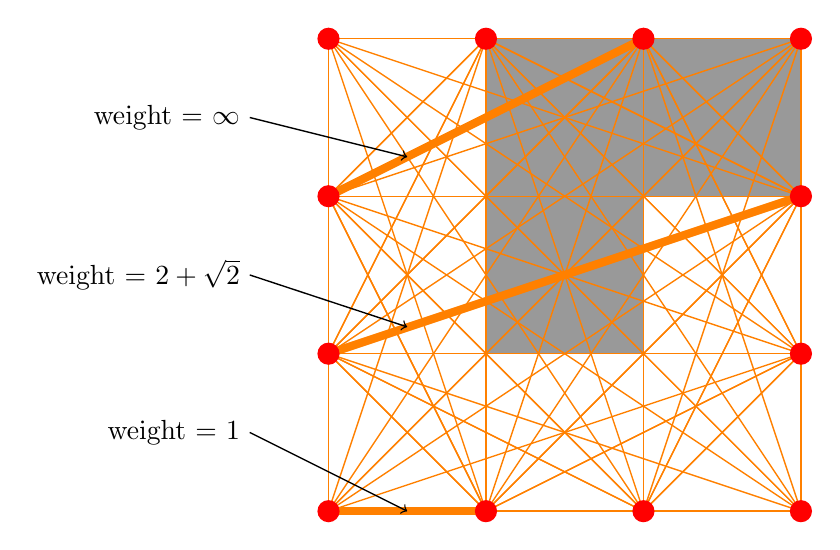
\begin{tikzpicture}[scale=2,line width=0.5pt]
    
      \filldraw[color=black!60,fill=black!40] (1,1) rectangle (2,3); 
      \filldraw[color=black!60,fill=black!40] (1,2) rectangle (3,3); 
  
      \foreach \x in {0,1,2,3} {
        \foreach \y in {0} {
          \foreach \a in {0,1,2,3} {
            \foreach \b in {3} {
              \draw[orange] (\x,\y) -- (\a,\b);
              \draw[orange] (\y,\x) -- (\b,\a);
            }
          }
        }
      }
      
      \foreach \x in {1,2} {
        \foreach \y in {0,3} {
          \foreach \a in {0,3} {
            \foreach \b in {1,2} {
              \draw[orange] (\x,\y) -- (\a,\b);
              \draw[orange] (\y,\x) -- (\b,\a);
            }
          }
        }
      }
      
      \draw[orange, line width = 3pt] (0,0) -- (1,0);
      \draw[orange, line width = 3pt](0,1) -- (3,2);
      \draw[orange, line width = 3pt] (0,2) -- (2,3);
      
      \node[left] at (-0.5,0.5) {weight = $1$};
      \draw[->] (-0.5,0.5) -- (0.5,0);
      \node[left] at (-0.5,1.5) {weight = $2 + \sqrt 2$};
      \draw[->] (-0.5,1.5) -- (0.5,1.17);
      \node[left] at (-0.5,2.5) {weight = $\infty$};
      \draw[->] (-0.5,2.5) -- (0.5,2.25);
      
      \fill[red] (0,0) circle (2pt);
      \fill[red] (0,1) circle (2pt);
      \fill[red] (0,2) circle (2pt);
      \fill[red] (0,3) circle (2pt);
      \fill[red] (3,0) circle (2pt);
      \fill[red] (3,1) circle (2pt);
      \fill[red] (3,2) circle (2pt);
      \fill[red] (3,3) circle (2pt);
      \fill[red] (1,0) circle (2pt);
      \fill[red] (2,0) circle (2pt);
      \fill[red] (1,3) circle (2pt);
      \fill[red] (2,3) circle (2pt);
      
     
    \end{tikzpicture}
    \caption[Anatomy of a block]{A block of size $3^{2}$ laid over the area of map it represents, with certain highlighted edge weights labeled.}
  %\label{fig:fig}
\end{figure}

\noindent
The edge weights for regular blocks are discovered by querying the {\em Local Distance Database (LDDB)}, which is introduced in the next subsection. Since the {\em LDDB} only contains data for regular blocks, the weights of edges in $B_{start}$ and $B_{goal}$ are calculated separately --- this is discussed in the Implementation chapter of this dissertation.\\

\noindent
Each block $B_{i,j}$ contains nodes that are collocational with nodes from up to six neighbouring blocks. {\em Block A*} maintains the invariant for two collocational nodes $n$ and $n'$ that $n.g = n'.g$ and $n.h = n'.h$.\\

\noindent
{\bfseries Local Distance Database --- $LDDB$}\\
\noindent
An $LDDB_{N}$ is a pre-computed database that holds the path length and inflection points of the optimum paths between all pairs of locations $(a,b)$ and $(c,d)$ for all map configurations $M$ of size $N^{2}$, where $a,b,c,d \in \mathbb{Z}^{2}$ and $(a,b)$ and $(c,d)$ lie on the boundary of $M$.\\

\noindent
{\bfseries Initialisation}\\
\noindent
For all $n \in B_{start}$, $n.g$ is set to $(n_{start},n).weight$. For all $n \in B_{goal}$, $n.h$ is set to $(n,n_{goal}).weight$. $B_{start}$ and $B_{goal}$ are treated as special cases as there is no guarantee that $start$ and $goal$ lie on the boundary of a block. The exceptional case that $B_{start} = B_{goal}$ must also be checked for.\\

\noindent
Having initialised $B_{start}$ and $B_{goal}$, $B_{start}$ is added to $openSet$.\\

\noindent
{\bfseries Iteration}\\
\noindent
The iteration stage of {\em Block A*} proceeds similarly to {\em A*}, though {\em Block A*} expands blocks chosen from $openSet_{blocks}$ whereas {\em A*} expands nodes. However, note that a block can be expanded multiple times, whereas in {\em A*} a node is only expanded once\footnote{This subtlety caused me such confusion that I eventually emailed Peter Yap, the author of the Block A* paper, for clarification. He explained the difference, and told me that he had included an explanation of this specific point when he gave a presentation [citation] on Block A* as the confusion is not uncommon.}. For this reason, a $length$ variable is maintained, which ensures that the algorithm terminates only when it is impossible to find a shorter path.\\

\noindent
{\bfseries Expansion}\\
\noindent
On expansion of $B_{i,j}$, {\em Block A*} attempts to relax every edge $e=(n_{ingress},n_{egress}) \in E_{i,j}$, where $n_{ingress} \in openSet_{i,j}$ and $n_{egress} \in V_{i,j}$. If $e$ is relaxed, all nodes that are collocational with $n_{egress}$ are added to the $openSet_{k,l}$ of their respective block $B_{k,l}$, and $B_{k,l}$ is added to $openSet$ if it is not already a member. \\

\noindent
{\bfseries Termination}\\
\noindent
The {\em h-value} of $B_{goal}$ is the actual shortest path from each node $n \in V_{goal}$, (see `Initialisation' section) as opposed to a Euclidean estimate that is used for the {\em h-value} in every other block. Therefore, if $B_{goal}.heapValue$ is less than the $heapValue$ of any other blocks in $openSet$ then there are no possible shorter paths to $B_{goal}$, so the algorithm terminates. This condition is ensured by the $length$ variable.\\

\noindent
{\bfseries Traceback}\\
\noindent
When {\em Block A*} terminates, the boundary nodes of the blocks through which $P_{G}$ passes can be found by recursively following the $parent$ pointers from $n_{goal}$ to $n_{start}$. See figure 2.8 (b). However, to recover the nodes of $P_{G}$ that do not lie on the boundaries of blocks, a traceback stage is required which involves multiple queries to the $LDDB$. See figure 2.8 (c). Although the details of this are not presented in Yap's paper, an explanation is presented in the Implementation chapter of this dissertation.\\

\begin{algorithm}
  \SetAlgoLined\DontPrintSemicolon
  \SetKwFunction{bAS}{BlockAStar}\SetKwFunction{expand}{Expand}\SetKwFunction{traceback}{TraceBack}
  \SetKwProg{myDef}{def}{}{}
  \myDef{\bAS{G, $n_{start}$, $n_{goal}$}}{
  \nl $B_{start} \gets init(n_{start})$\;
  \nl $B_{goal} \gets init(n_{goal})$\;
  \nl $length \gets \infty$\;
  \nl $openSet_{blocks}.add(B_{start})$\;
  \nl \While{$(openSet_{blocks} \neq \bot) \land ((openSet_{blocks}.peek()).heapValue < length)$} {
    \nl $B_{curr} \gets openSet_{blocks}.pop()$\;
    \nl $openSet_{curr} \gets B_{curr}.openSet$\;
    \nl \If{$B_{curr} = B_{goal}$} {
      \nl $length \gets \min\limits_{n \in openSet_{curr}} (n.g + euclidean(n,n_{goal}),length)$\;
    }
    \nl $\expand(B_{curr},openSet_{curr})$\;
  }
  \nl \uIf{$length \neq \infty$}{
    \nl $\traceback(n_{goal})$\;
  } \nl \Else {
     \nl \KwRet{$\bot$}\;
  }
}{}

 \setcounter{AlgoLine}{0}
  \myDef{\expand{$B_{curr},openSet_{curr}$}}{
    \nl \While{$openSet_{curr} \neq \bot $}{
      \nl $n_{ingress} \gets openSet_{curr}.pop()$\;
      \nl \ForEach{$n_{egress} \in B_{curr}$}{
        \nl \uIf{$n_{ingress}.g + (n_{ingress},n_{egress}).weight < n_{egress}.g$} {
          \nl $n_{egress}.g \gets n_{ingress}.g + (n_{ingress},n_{egress}).weight$\;
            \nl \ForEach{$n' \in n_{egress}.collocational$}{
              \nl $n' \gets n_{ingress}.g + (n_{ingress},n_{egress}).weight$\;
              \nl $openSet_{n'.coord}.add(n')$\;
              \nl \uIf{$openSet_{blocks}.contains(B_{n'.coord}) = false$} {
                \nl $openSet_{blocks}.add(B_{n'.coord})$\;
              }
            }
        }
      }
    }
  }
 
  \caption{{\sc Block A*}}
\end{algorithm} 


\begin{figure}
    \centering
    \begin{tikzpicture}
    
\node (a) at (0,10) {
    	\begin{tikzpicture}[scale=0.85,line width=0.5pt]
	      	\filldraw[color=black!60,fill=black!40] (0,0) rectangle (2,3); 
		\filldraw[color=black!60,fill=black!40] (1,7) rectangle (8,8); 
		\filldraw[color=black!60,fill=black!40] (7,7) rectangle (8,5); 
		\filldraw[color=black!60,fill=black!40] (2,4) rectangle (5,6);
		\filldraw[color=black!60,fill=black!40] (3,2) rectangle (5,4); 
		\filldraw[color=black!60,fill=black!40] (4,1) rectangle (5,2);  
     	 	\draw[color=black!60] (0,0) grid (9,9);
      		\draw[black] (0,0) -- (0,9);
      		\draw[black] (0,0) -- (9,0);
      		\draw[black] (9,9) -- (0,9);
      		\draw[black] (9,9) -- (9,0);
		\fill[blue] (1,4) circle (3pt);
		\node[below left] at (1,4) {$start$};
		\fill[blue] (8,2) circle (3pt);
		\node[below left] at (8,2) {$goal$};
		
		\node at (4.5,-1) {(a) Original map $M$};
	    \end{tikzpicture}
	    };	   
	   
\node (a) at (0,0) {
    	    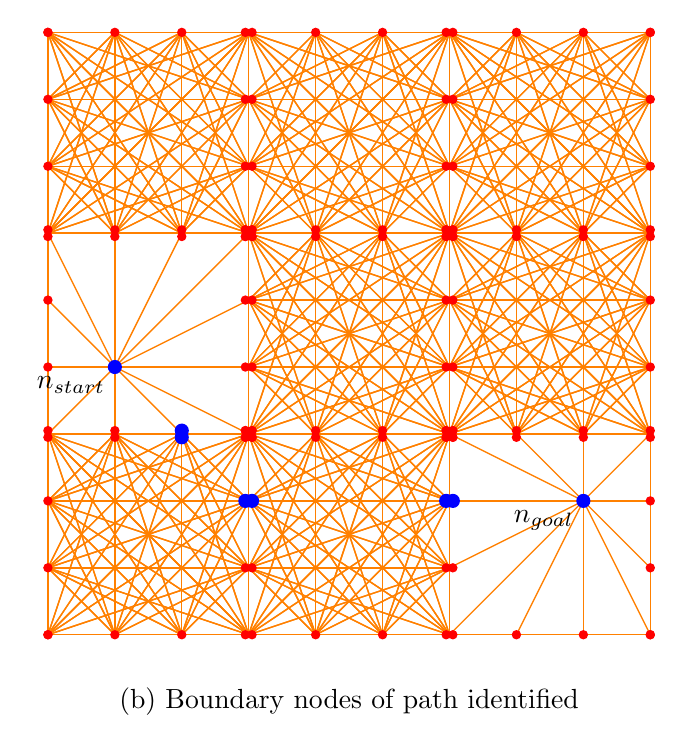
\begin{tikzpicture}[scale=0.85,line width=0.5pt]
  
      \foreach \i in {0,3,6} {
      \foreach \j in {0,3,6} {
      \foreach \x in {0,1,2,3} {
        \foreach \y in {0,3} {
          \foreach \a in {0,1,2,3} {
            \foreach \b in {0,3} {
             \pgfmathparse{int(\x + \i)};
             \let\xn\pgfmathresult;
             \pgfmathparse{int(\a + \i)};
             \let\an\pgfmathresult;
             \pgfmathparse{int(\y + \j)};
             \let\yn\pgfmathresult;
             \pgfmathparse{int(\b + \j)};
             \let\bn\pgfmathresult;
              \draw[orange] (\xn,\yn) -- (\an,\bn);
              \draw[orange] (\yn,\xn) -- (\bn,\an);
            }
          }
        }
      }
      }}
      
      \foreach \i in {0,3,6} {
      \foreach \j in {0,3,6} {
      \foreach \x in {1,2} {
        \foreach \y in {0,3} {
          \foreach \a in {1,2} {
            \foreach \b in {0,3} {
             \pgfmathparse{int(\x+\i)};
             \let\xn\pgfmathresult;
             \pgfmathparse{int(\a+\j)};
             \let\an\pgfmathresult;
             \pgfmathparse{int(\y+\j)};
             \let\yn\pgfmathresult;
             \pgfmathparse{int(\b+\i)};
             \let\bn\pgfmathresult;
              \draw[orange] (\xn,\yn) -- (\bn,\an);
              \draw[orange] (\yn,\xn) -- (\an,\bn);
            }
          }
        }
      }
      }}
      
      \filldraw[color=orange, fill=white] (0,3) rectangle (3,6);
      \filldraw[color=orange, fill=white] (6,0) rectangle (9,3);
      
      \draw[orange] (1,4) -- (0,3);
      \draw[orange] (1,4) -- (0,4);
      \draw[orange] (1,4) -- (0,5);
      \draw[orange] (1,4) -- (0,6);
      \draw[orange] (1,4) -- (3,3);
      \draw[orange] (1,4) -- (3,4);
      \draw[orange] (1,4) -- (3,5);
      \draw[orange] (1,4) -- (3,6);
      \draw[orange] (1,4) -- (1,3);
      \draw[orange] (1,4) -- (2,3);
      \draw[orange] (1,4) -- (1,6);
      \draw[orange] (1,4) -- (2,6);

      \draw[orange] (8,2) -- (6,0);
      \draw[orange] (8,2) -- (6,1);
      \draw[orange] (8,2) -- (6,2);
      \draw[orange] (8,2) -- (6,3);
      \draw[orange] (8,2) -- (9,0);
      \draw[orange] (8,2) -- (9,1);
      \draw[orange] (8,2) -- (9,2);
      \draw[orange] (8,2) -- (9,3);
      \draw[orange] (8,2) -- (7,0);
      \draw[orange] (8,2) -- (8,0);
      \draw[orange] (8,2) -- (7,3);
      \draw[orange] (8,2) -- (8,3);     
      
      \fill[red] (1,4) circle (2pt);
      \node[below left] at (1,4) {$n_{start}$};
      \fill[red] (8,2) circle (2pt);
      \node[below left] at (8,2) {$n_{goal}$};
      
      \foreach \x in {0,1,2,2.95,3.05,4,5,5.95,6.05,7,8,9} {
        \foreach \y in {0,9} {
              \fill[red] (\x,\y) circle (2pt);
              \fill[red] (\y,\x) circle (2pt);
        }
      }
      
      \foreach \x in {1,2,4,5,7,8} {
        \foreach \y in {3,6} {
          \pgfmathparse{(\y + 0.05)};
           \let\ya\pgfmathresult;
            \pgfmathparse{(\y - 0.05)};
           \let\yb\pgfmathresult;
              \fill[red] (\x,\ya) circle (2pt);
              \fill[red] (\x,\yb) circle (2pt);
              \fill[red] (\ya,\x) circle (2pt);
              \fill[red] (\yb,\x) circle (2pt);
        }
      }
      
       \foreach \x in {3,6} {
        \foreach \y in {3,6} {
          \pgfmathparse{(\x + 0.05)};
           \let\xa\pgfmathresult;
            \pgfmathparse{(\x - 0.05)};
           \let\xb\pgfmathresult;
           \pgfmathparse{(\y + 0.05)};
           \let\ya\pgfmathresult;
              \fill[red] (\xa,\ya) circle (2pt);
              \fill[red] (\xb,\ya) circle (2pt);
              \fill[red] (\ya,\xa) circle (2pt);
              \fill[red] (\ya,\xb) circle (2pt);
        }
      }
      
             \foreach \x in {3,6} {
        \foreach \y in {3,6} {
          \pgfmathparse{(\x + 0.05)};
           \let\xa\pgfmathresult;
            \pgfmathparse{(\x - 0.05)};
           \let\xb\pgfmathresult;
           \pgfmathparse{(\y - 0.05)};
           \let\ya\pgfmathresult;
              \fill[red] (\xa,\ya) circle (2pt);
              \fill[red] (\xb,\ya) circle (2pt);
              \fill[red] (\ya,\xa) circle (2pt);
              \fill[red] (\ya,\xb) circle (2pt);
        }
      }
      
      \fill[blue] (1,4) circle (3pt);
      \fill[blue] (2,3.05) circle (3pt);
      \fill[blue] (2,2.95) circle (3pt);
      \fill[blue] (2.95,2) circle (3pt);
      \fill[blue] (3.05,2) circle (3pt);
      \fill[blue] (5.95,2) circle (3pt);
      \fill[blue] (6.05,2) circle (3pt);
      \fill[blue] (8,2) circle (3pt);
      
      \node at (4.5,-1) {(b) Boundary nodes of path identified};
     
    \end{tikzpicture}
	    };
	    
\node (a) at (10,10) {
    	    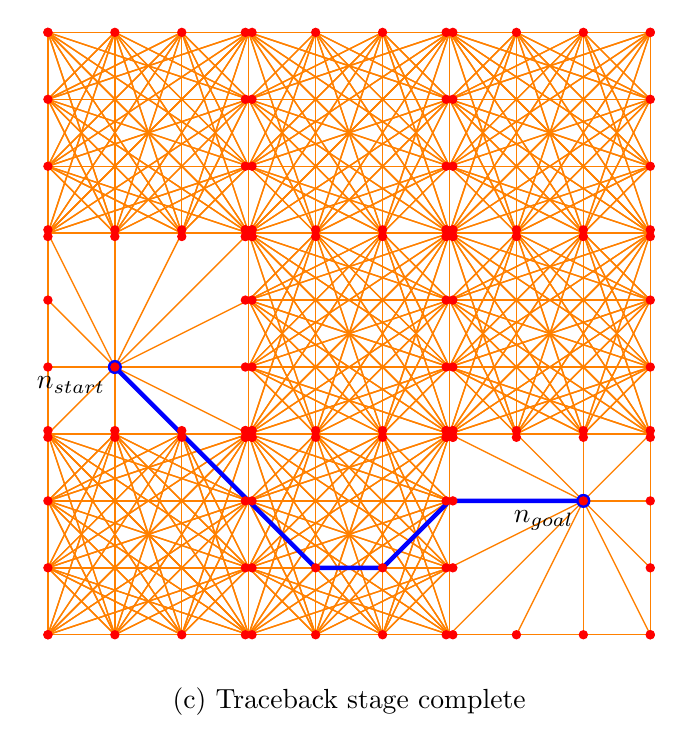
\begin{tikzpicture}[scale=0.85,line width=0.5pt]
  
      \foreach \i in {0,3,6} {
      \foreach \j in {0,3,6} {
      \foreach \x in {0,1,2,3} {
        \foreach \y in {0,3} {
          \foreach \a in {0,1,2,3} {
            \foreach \b in {0,3} {
             \pgfmathparse{int(\x + \i)};
             \let\xn\pgfmathresult;
             \pgfmathparse{int(\a + \i)};
             \let\an\pgfmathresult;
             \pgfmathparse{int(\y + \j)};
             \let\yn\pgfmathresult;
             \pgfmathparse{int(\b + \j)};
             \let\bn\pgfmathresult;
              \draw[orange] (\xn,\yn) -- (\an,\bn);
              \draw[orange] (\yn,\xn) -- (\bn,\an);
            }
          }
        }
      }
      }}
      
      \foreach \i in {0,3,6} {
      \foreach \j in {0,3,6} {
      \foreach \x in {1,2} {
        \foreach \y in {0,3} {
          \foreach \a in {1,2} {
            \foreach \b in {0,3} {
             \pgfmathparse{int(\x+\i)};
             \let\xn\pgfmathresult;
             \pgfmathparse{int(\a+\j)};
             \let\an\pgfmathresult;
             \pgfmathparse{int(\y+\j)};
             \let\yn\pgfmathresult;
             \pgfmathparse{int(\b+\i)};
             \let\bn\pgfmathresult;
              \draw[orange] (\xn,\yn) -- (\bn,\an);
              \draw[orange] (\yn,\xn) -- (\an,\bn);
            }
          }
        }
      }
      }}
      
      \filldraw[color=orange, fill=white] (0,3) rectangle (3,6);
      \filldraw[color=orange, fill=white] (6,0) rectangle (9,3);
      
      \draw[orange] (1,4) -- (0,3);
      \draw[orange] (1,4) -- (0,4);
      \draw[orange] (1,4) -- (0,5);
      \draw[orange] (1,4) -- (0,6);
      \draw[orange] (1,4) -- (3,3);
      \draw[orange] (1,4) -- (3,4);
      \draw[orange] (1,4) -- (3,5);
      \draw[orange] (1,4) -- (3,6);
      \draw[orange] (1,4) -- (1,3);
      \draw[orange] (1,4) -- (2,3);
      \draw[orange] (1,4) -- (1,6);
      \draw[orange] (1,4) -- (2,6);

      \draw[orange] (8,2) -- (6,0);
      \draw[orange] (8,2) -- (6,1);
      \draw[orange] (8,2) -- (6,2);
      \draw[orange] (8,2) -- (6,3);
      \draw[orange] (8,2) -- (9,0);
      \draw[orange] (8,2) -- (9,1);
      \draw[orange] (8,2) -- (9,2);
      \draw[orange] (8,2) -- (9,3);
      \draw[orange] (8,2) -- (7,0);
      \draw[orange] (8,2) -- (8,0);
      \draw[orange] (8,2) -- (7,3);
      \draw[orange] (8,2) -- (8,3);   
      
      \draw[blue,ultra thick] (1,4) -- (2,3) -- (3,2) -- (4,1) -- (5,1) -- (6,2) -- (8,2);
      \fill[blue] (1,4) circle (3pt);
      \fill[blue] (8,2) circle (3pt);
      \fill[red] (4,1) circle (2pt);
      \fill[red] (5,1) circle (2pt);
      
      \fill[red] (1,4) circle (2pt);
      \node[below left] at (1,4) {$n_{start}$};
      \fill[red] (8,2) circle (2pt);
      \node[below left] at (8,2) {$n_{goal}$};
      
      \foreach \x in {0,1,2,2.95,3.05,4,5,5.95,6.05,7,8,9} {
        \foreach \y in {0,9} {
              \fill[red] (\x,\y) circle (2pt);
              \fill[red] (\y,\x) circle (2pt);
        }
      }
      
      \foreach \x in {1,2,4,5,7,8} {
        \foreach \y in {3,6} {
          \pgfmathparse{(\y + 0.05)};
           \let\ya\pgfmathresult;
            \pgfmathparse{(\y - 0.05)};
           \let\yb\pgfmathresult;
              \fill[red] (\x,\ya) circle (2pt);
              \fill[red] (\x,\yb) circle (2pt);
              \fill[red] (\ya,\x) circle (2pt);
              \fill[red] (\yb,\x) circle (2pt);
        }
      }
      
       \foreach \x in {3,6} {
        \foreach \y in {3,6} {
          \pgfmathparse{(\x + 0.05)};
           \let\xa\pgfmathresult;
            \pgfmathparse{(\x - 0.05)};
           \let\xb\pgfmathresult;
           \pgfmathparse{(\y + 0.05)};
           \let\ya\pgfmathresult;
              \fill[red] (\xa,\ya) circle (2pt);
              \fill[red] (\xb,\ya) circle (2pt);
              \fill[red] (\ya,\xa) circle (2pt);
              \fill[red] (\ya,\xb) circle (2pt);
        }
      }
      
             \foreach \x in {3,6} {
        \foreach \y in {3,6} {
          \pgfmathparse{(\x + 0.05)};
           \let\xa\pgfmathresult;
            \pgfmathparse{(\x - 0.05)};
           \let\xb\pgfmathresult;
           \pgfmathparse{(\y - 0.05)};
           \let\ya\pgfmathresult;
              \fill[red] (\xa,\ya) circle (2pt);
              \fill[red] (\xb,\ya) circle (2pt);
              \fill[red] (\ya,\xa) circle (2pt);
              \fill[red] (\ya,\xb) circle (2pt);
        }
      }
      
      \node at (4.5,-1) {(c) Traceback stage complete};
      
     
    \end{tikzpicture}
	    };
	    
\node (a) at (10,0) {
    	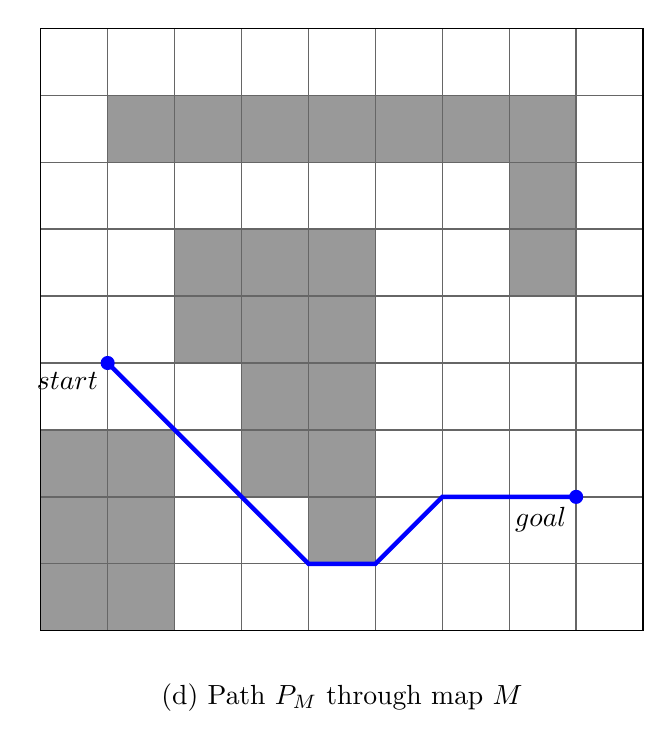
\begin{tikzpicture}[scale=0.85,line width=0.5pt]
	      	\filldraw[color=black!60,fill=black!40] (0,0) rectangle (2,3); 
		\filldraw[color=black!60,fill=black!40] (1,7) rectangle (8,8); 
		\filldraw[color=black!60,fill=black!40] (7,7) rectangle (8,5); 
		\filldraw[color=black!60,fill=black!40] (2,4) rectangle (5,6);
		\filldraw[color=black!60,fill=black!40] (3,2) rectangle (5,4); 
		\filldraw[color=black!60,fill=black!40] (4,1) rectangle (5,2);  
     	 	\draw[color=black!60] (0,0) grid (9,9);
      		\draw[black] (0,0) -- (0,9);
      		\draw[black] (0,0) -- (9,0);
      		\draw[black] (9,9) -- (0,9);
      		\draw[black] (9,9) -- (9,0);
		\node[below left] at (1,4) {$start$};
		\node[below left] at (8,2) {$goal$};
		\fill[blue] (1,4) circle (3pt);
      		\fill[blue] (8,2) circle (3pt);
      		\draw[blue,ultra thick] (1,4) -- (2,3) -- (3,2) -- (4,1) -- (5,1) -- (6,2) -- (8,2);
		
		\node at (4.5,-1) {(d) Path $P_{M}$ through map $M$};
	    \end{tikzpicture}
	    };	

    \end{tikzpicture}
    \caption[Solution of {\em Block A*}]{Solution of {\em Block A*}}
  %\label{fig:fig}
\end{figure}


\clearpage
\section {Requirements analysis}

As specified in the {\bfseries Work to be done} section of the Proposal (see {\bfseries Appendix E}), this project is logically composed of four parts. This section outlines the functional and non-functional requirements for each part, and their relative priorities using the MoSCoW system. \\
\centerline {{\bf M} - Must; {\bf S} - Should; {\bf C} - Could; {\bf W} - Won't}

\subsection{Testing simulator}

\begin{center}
    \begin{tabular}{ l | p{10cm} | l}
    ID & Functional requirement & Priority  \\ \hline
    1 & The system shall load one of a collection of maps from the generator & M \\ \hline
    2 & The system shall load one of a collection of maps from a saved file & S \\ \hline
    3 & The system shall create a grid-graph from a given map & M \\ \hline
    4 & The system shall create a visibility graph from a given map & C \\ \hline
    5 & The system shall run one of a collection of any-angle path-finding algorithms on a graph and collect data such as the path-length and the length of computation & M \\ \hline
    6 & The system shall display a visual representation of the current map and the paths found by any algorithms that have been run on it & M \\ \hline
    7 & The system shall display the numeric statistics for each path for the current map & M \\ \hline
     \hline 
    ID & Non-functional requirement & Priority  \\ \hline
    1 & The system shall be designed in a modular way to allow easy extension for new algorithms & S \\
    \end{tabular}
\end{center}

\subsection{Map generation}

\begin{center}
    \begin{tabular}{ l | p{10cm} | l }
    ID & Functional requirement & Priority  \\ \hline
    1 & The system shall generate pseudo-random maps of a given resolution, coverage percentage and clustering & M \\ \hline
    2 & The system shall allow maps to be saved so that multiple tests can be run on the same map suite & M \\ \hline
     3 & The system shall allow maps to be created with an interactive map editor & C\\ \hline
          \hline 
    ID & Non-functional requirement & Priority  \\ \hline
    1 & The system shall generate maps of the highest resolution in under 2 seconds & S \\
    \end{tabular}
\end{center}
	
\subsection{Algorithm implementation}

\begin{center}
    \begin{tabular}{ l | p{10cm} | l}
    ID & Functional requirement & Priority  \\ \hline
    1 & The system shall correctly implement each of the chosen algorithms. If a path exists, the path and numerical statistics will be returned. If no path exists, this will be returned   & M \\ \hline
    2 & The system shall allow arbitrary start and end coordinates for any map & S \\ \hline
     \hline 
    ID & Non-functional requirement & Priority  \\ \hline
    1 & The system shall be designed in a modular way to allow easy extension for new algorithms & S \\
    \end{tabular}
\end{center}

\subsection{Data gathering}

\begin{center}
    \begin{tabular}{ l | p{10cm} | l}
    ID & Functional requirement & Priority  \\ \hline
    1 & The system shall write statistics for an arbitrary set of specified algorithms on an arbitrary set of specified maps and write the results to a CSV file & M \\ \hline
     \hline 
    ID & Non-functional requirement & Priority  \\ \hline
    1 & The system shall be designed with a clear API that enables quick and easy data gathering. & M \\
    \end{tabular}
\end{center}

\noindent
\missingfigure{UML diagrams - use case and sequence diagram etc}

\section {Testing}

A thorough testing strategy was devised to reduce the chances of bugs being introduced into the code. Separate strategies were required for different modules of the system:

\begin{description}
\item[Simulator]\hfil \\
{\em Core structural classes} --- basic functionality to be unit tested;\\
{\em Line of sight algorithm} --- to be unit tested thoroughly, as its correctness will be assumed during testing of pathfinding algorithm implementations;\\
{\em Pathfinding algorithms} --- correctness of all paths returned by to be optionally verified.
\end{description}
\begin{description}
\item[User interface]\hfil \\
{\em Use case scenarios} --- to be manually tested by human user.
\end{description}
\begin{description}
\item[Data extraction scripts]\hfil \\
{\em Exported CSVs} --- contents of CSV files to be unit tested.
\end{description}

\section {Design model}

\noindent
Once the preparation phase of the project was completed, the plan for the implementation phase was refined from that presented in the Project Proposal (see Appendix ?). An incremental model of implementation was adopted, with new modules being developed and tested separately before being integrated into the work program. The milestones of the project were:
\begin{description}
\item[Milestone 1]\hfil \\
Maps of arbitrary size, coverage and clustering can be created and printed to system output.
\item[Milestone 2]\hfil \\
Arbitrary maps can be converted to graphs, and {\em Dijkstra} and {\em A*} can be run on these maps. A visual representation of the path can be printed to system output.
\item[Milestone 3]\hfil \\
Basic UI is built, including all functionality from {\bfseries Milestone 2}. Basic path statistics are displayed.
\item[Milestone 4]\hfil \\
Map saving, map loading and map creation functionality are present. This will facilitate debugging edge cases for more complex algorithms.
\item[Milestone 5]\hfil \\
{\em A* with post-smoothing}, {\em Theta*} and {\em Lazy Theta*} are implemented.
\item[Milestone 6]\hfil \\
{\em Block A*} is implemented.
\item[Milestone 7]\hfil \\
Data extraction scripts are implemented.
\end{description}

\section {Languages and tools}

This section justifies the languages, libraries and tools that were chosen for this project.

\begin{description}
  \item[Programming language] \hfill \\
  {\em Java} --- provides abstraction and class hierarchy to enable development of modular, extensible code.
  \item[Libraries] \hfill \\
  {\em Swing} --- for graphical user interface design;\\ 
  {\em CSVWriter} --- for data export.\\
  {\em JUnit} --- for unit testing.
  \item[Integrated development environment] \hfill \\
  {\em Eclipse} --- allows rapid development through integrated testing, refactoring and version control tools.
  \item[Statistical analysis and visualisation] \hfill \\
  {\em R} --- open-source statistical package; chosen due to its flexibility and extensibility.
  \item[Document preparation] \hfill \\
  {\LaTeX} --- allows precise, integrated control over all aspects of document layout and style;\\
  {\em Tikz} --- drawing package for \LaTeX\ that enables programmable diagram creation;\\
  {\em algorithm2e} --- pseudo-code package for \LaTeX\ that enables integration with the parent document.
  \item[Backup] \hfill \\
  {\em DropBox} and {\em Google Drive} --- maintain multiple shadow copies of my work in the cloud.
  \item[Version Control]\hfill \\
  {\em GitHub} --- facilitated exploring different implementation strategies by forking my core code repository.
  
\end{description}

%\cleardoublepage
\chapter{Implementation}

This chapter provides an overview of the implementation of the project, and investigates some of its more interesting features.\\

\noindent
The chapter is split into six parts: 
\begin{description}
  \item{\bf Map generation}\\ \hfill  an explanation of the algorithm used to generate maps.
  \item{\bf Simulation}\\ \hfill an overview of the simulator, including graph generation and algorithm data.
  \item{\bf Algorithms}\\ \hfill details of the implementation of each of the pathfinding algorithms, with specific attention given to {\em Block A*}.
  \item{\bf User Interface}\\ \hfill an overview of the graphical user interface. 
  \item{\bf Data extraction}\\ \hfill an explanation of how large volumes of data are extracted for statistical analysis.
  \item{\bf Testing}\\ \hfill an overview of the methods to test the code for correctness.
  \end{description}

\begin{figure}
  \centering
  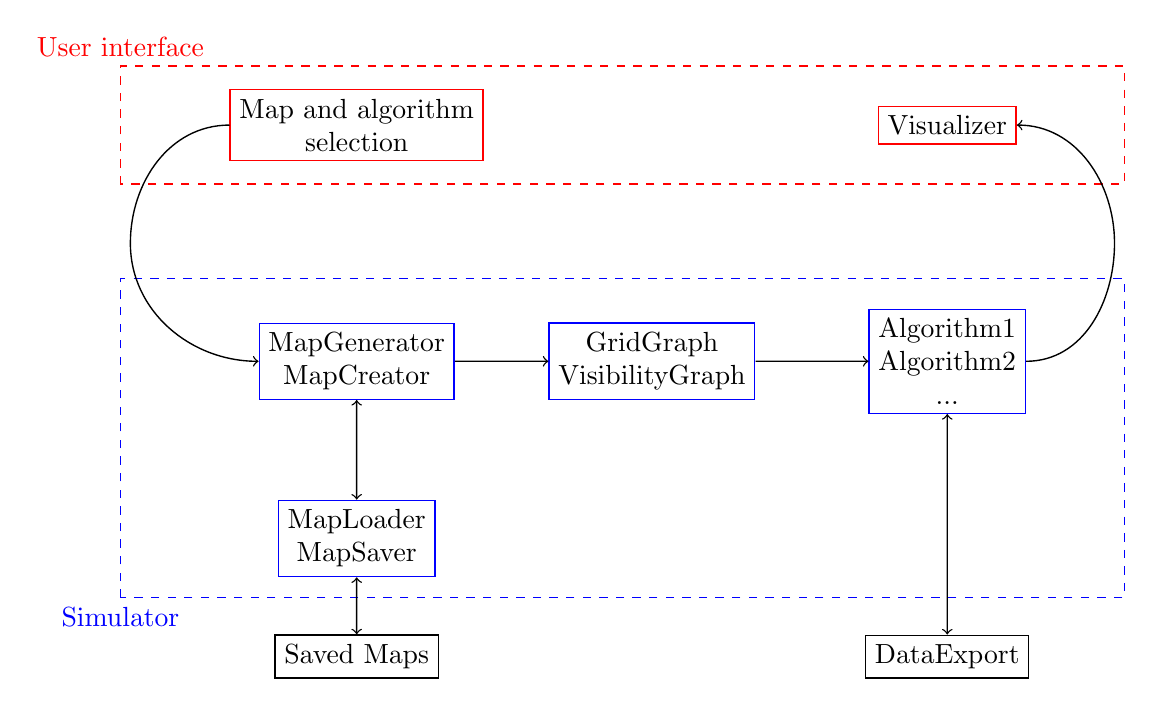
\begin{tikzpicture}[scale=0.75,line width=0.5pt]
  \filldraw[color=red,fill=white,dashed] (0,5) rectangle (17,7); 
  \node[above, red] at (0,7) {User interface};
  \filldraw[color=blue,fill=white,dashed] (0,-2) rectangle (17,3.4); 
  \node[below, blue] at (0,-2) {Simulator};
  
\node[draw=red,shape=rectangle,align=center] at (4,6) (1) {Map and algorithm \\selection};
\node at (0,4) (2) {};
\node[draw=blue,shape=rectangle,align=center] at (4,2) (3) {MapGenerator\\MapCreator};
\node[draw=blue,shape=rectangle,align=center] at (9,2) (4) {GridGraph\\VisibilityGraph};
\node[draw=blue,shape=rectangle,align=center] at (14,2) (5) {Algorithm1\\Algorithm2\\...};
\node at (17,4) (6) {};
\node[draw=red,shape=rectangle,align=center] at (14,6) (7) {Visualizer};
\node[draw=blue,shape=rectangle,align=center] at (4,-1) (8) {MapLoader\\MapSaver};
\node[draw=black,shape=rectangle,align=center] at (4,-3) (9) {Saved Maps};
\node[draw=black,shape=rectangle,align=center] at (14,-3) (10) {DataExport};

\draw[->] (1.west) to[out=180,in=90] (2.east) to[out=-90,in=180] (3.west);
\draw[->] (3) to (4);
\draw[->] (4) to (5);
\draw[->] (5.east) to[out=0,in=-90] (6.west) to[out=90,in=0] (7.east);
\draw[<->] (3) to (8);
\draw[<->] (8) to (9);
\draw[<->] (5) to (10);


  \end{tikzpicture}
  \caption{Flow of the user interface and simulator} 
  \label{fig:lineofsight}
\end{figure}

\newpage
\section{Map generation}

In order to reach reliable conclusions about the performance of the algorithms, a method was required to generate large volumes of maps of a given size $N^{2}$, coverage percentage $C$ and clustering $D$ was require. A bespoke was devised for this project to pseudo-randomly create such maps. The algorithm creates maps of a specified level of clustering by loosely approximating the idea of potential fields.\\

\noindent
The input to the algorithm includes an integer matrix $m_{i,j}$ of size $N^{2}$ - where each element has been initialised to value 1. At any point in the algorithm, $m_{i,j}$'s value represents its `potential' - i.e. the chance that $m_{i,j}$ will be the next element set to 0 (i.e. blocked). The algorithm performs $C \times N^{2}$ iterations. In each iteration, it chooses a random number $r$ between $0$ and $\sum\limits_{i,j} m_{i,j}$. It then traverses the matrix row-by-row until the sum of the elements it has seen is at least $r$. The potential of the element that has been reached is set to $0$, and the potential of the surrounding elements is increased in a crude approximation of a potential field. The output is an integer matrix $m_{i,j}$ of size $N^{2}$ - where $C\%$ of the elements have value 0, which denotes a blocked cell \footnote{Note that this is not the same as our notation in the Preparation chapter, where a 0 denoted a free cell. The notation of 0 denoting a blocked cell is {\em only} used during the execution of the map generation algorithm.}, and the rest of the elements have value \textgreater $0$, which denotes a free cell. The array can then be parsed into a {\tt Map} by the {\tt Map} constructor.

\begin{algorithm}[htp]
  \SetAlgoLined\DontPrintSemicolon
  \SetKwFunction{genMap}{GenerateMap} \SetKwFunction{setBlocked}{SetAsBlocked}
  \SetKwProg{myDef}{def}{}{}
  \myDef{\genMap{$m, C, D$}}{
    \nl \Repeat{$(C\times N^{2}) times$} {
      \nl $r \gets random(0,\sum\limits_{i,j} m_{i,j})$\;
      \nl $i,j \gets 0$\;
      \nl \While{$r\geq 0$} {
        \nl $r \gets r - m_{i,j}$\;
        \nl \uIf{$i < R-1$} {
          \nl $i \gets i+1$\;
        } \nl \Else {
          \nl $i \gets 0$\;
          \nl $j \gets j+1$\;
        }
     }
     \nl \setBlocked{$i,j$};     
  }
  }
  \myDef{\setBlocked{$m_{i,j}$}} {
    \nl $m_{i,j} \gets 0$\;
    \nl \ForEach {$m_{k,l}$ in $horizontalOrVerticalNeighbour(m_{i,j})$} {
      \nl \uIf{$m_{k,l} \neq 0$} {
        \nl $m_{k,l} \gets m_{k,l} + D$\;
      }
  }
  \nl \ForEach {$ m_{k,l}$ in  $diagonalNeighbour(m_{i,j})$} {
      \nl \uIf{$m_{k,l} \neq 0$} {
        $m_{k,l} \gets a_{k,l} + 2\times D$\;
      }
  }
}
\caption{{\sc GenerateMap}}
 \end{algorithm} 
 
 \begin{figure}[h]
\begin{subfigure}{.3\textwidth}
    \centering
    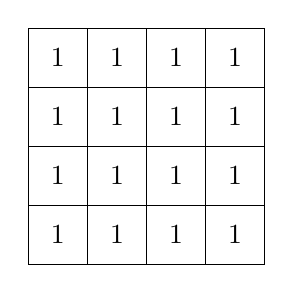
\begin{tikzpicture}[scale=0.75,line width=0.5pt]

     \draw (0,0) grid (4,4);
    
     \foreach \x in {0,1,2,3} {
        \foreach \y in {0,1,2,3} {
          \pgfmathparse{(\x + 0.5)};
          \let\xa\pgfmathresult;
          \pgfmathparse{\y + 0.5};
          \let\ya\pgfmathresult;
          \node at (\xa,\ya) {1};
        }
      }
           
    \end{tikzpicture}
    \caption{Initialisation}
    %\label{fig:sfig1}
  \end{subfigure}
  \begin{subfigure}{.3\textwidth}
    \centering
    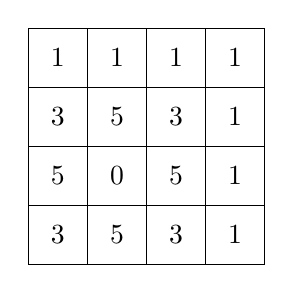
\begin{tikzpicture}[scale=0.75,line width=0.5pt]
     \draw (0,0) grid (4,4);
    
    \node at (0.5,0.5) {3};
    \node at (1.5,0.5) {5};
    \node at (2.5,0.5) {3};
    \node at (3.5,0.5) {1};
    \node at (0.5,1.5) {5};
    \node at (1.5,1.5) {0};
    \node at (2.5,1.5) {5};
    \node at (3.5,1.5) {1};
    \node at (0.5,2.5) {3};
    \node at (1.5,2.5) {5};
    \node at (2.5,2.5) {3};
    \node at (3.5,2.5) {1};
    \node at (0.5,3.5) {1};
    \node at (1.5,3.5) {1};
    \node at (2.5,3.5) {1};
    \node at (3.5,3.5) {1};
      
    \end{tikzpicture}
    \caption{Iteration 1: r = 5}
    %\label{fig:sfig1}
  \end{subfigure}
  %
  \begin{subfigure}{.3\textwidth}
    \centering
    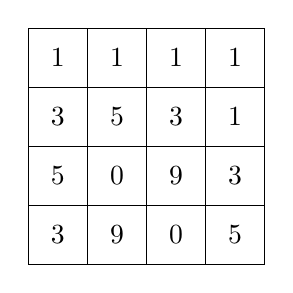
\begin{tikzpicture}[scale=0.75,line width=0.5pt]
    
    \draw (0,0) grid (4,4);
    
    \node at (0.5,0.5) {3};
    \node at (1.5,0.5) {9};
    \node at (2.5,0.5) {0};
    \node at (3.5,0.5) {5};
    \node at (0.5,1.5) {5};
    \node at (1.5,1.5) {0};
    \node at (2.5,1.5) {9};
    \node at (3.5,1.5) {3};
    \node at (0.5,2.5) {3};
    \node at (1.5,2.5) {5};
    \node at (2.5,2.5) {3};
    \node at (3.5,2.5) {1};
    \node at (0.5,3.5) {1};
    \node at (1.5,3.5) {1};
    \node at (2.5,3.5) {1};
    \node at (3.5,3.5) {1};
      
    \end{tikzpicture}
    \caption{Iteration 2: r = 2}
    %\label{fig:sfi2}
  \end{subfigure}
  \caption{Two iterations of {\tt GenerateMap} with $R$=4 and $D$=2}
  %\label{fig:fig}
\end{figure}

\newpage
\section{Simulation}

\subsection{Graph Generation}

To create a graph from a map, the map was iterated over twice. The first iteration created nodes for all the coordinates that were valid node locations. The second iteration set the neighbours of each node. Checks for both of the iterations were performed by checking whether neighbouring blocks were blocked. See Figure 3.3.\\

\begin{figure}
\begin{lstlisting}
...
Coordinate[] diagonalRelativeCellCoordinates = 
		{new Coordinate(-1,-1), new Coordinate(0,-1), 
		new Coordinate(0,0), new Coordinate(-1,0)};
		
Node[][] graphArray2D = 
	new Node[map.getWidth()+1][map.getHeight()+1];
for(int j=0; j < map.getHeight()+1; j++) {
	for(int i=0; i < map.getWidth()+1; i++) {
		boolean isUnblockedAdjacentCell = false;
		for(Coordinate c: diagonalRelativeCellCoordinates) {
			try {
				if(!map.getCell(i+c.getX(),j+c.getY()).isBlocked()) {
					isUnblockedAdjacentCell=true;
				}
			} catch (ArrayIndexOutOfBoundsException e) {}
		}
		if(!isUnblockedAdjacentCell) {
			graphArray2D[i][j] = null;
		} else {
			graphArray2D[i][j] = new Node(new Coordinate(i,j));
		}
	}
}
...
\end{lstlisting}
\caption{Code snippet showing {\tt Node} creation for grid-based graphs}
\end{figure}

\noindent
As discussed in the Preparation chapter, along with grid-based graphs, I am also going to investigate the performance benefits of running path-finding algorithms on visibility graphs. The creation of visibility graphs depends on having a {\tt LineOfSight} function.\\

\noindent
{\bf Line of Sight}\\

\noindent
The line of sight algorithm is based on the pseudocode in [reference Theta* paper], which itself is a derivative of Bresenham's line drawing algorithm - though instead of choosing pixels (i.e. cells) to draw, it chooses cells to check whether they are blocked. Bresenham's algorithm is a useful framework as it avoids any floating point calculations when the start and end points are integers - this has dual benefits:
\begin{itemize}
\item the algorithm is fast
\item the algorithm doesn't suffer from rounding errors inherent in floating-point calculations. 
\end{itemize}
\noindent
A notable alteration to the basic Bresenham algorithm is that instead of checking one cell per column (or one per row), the line of sight algorithm will check any cell that the real line passes through. This only requires a minor alteration.\\

\noindent
For the purposes of clarity, the pseudocode presented in {\sc LineOfSight} assumes the line of sight is in octant 1 - i.e. whose angle with the x-axis is between $0^{o}$ and $45^{o}$. The full pseudocode can be found in Appendix ?. On this assumption, the key variables are:
\begin{description}
\item{$x$ and $y$} - integers that represent the coordinate of the cell being considered, which is always a cell that the line passes through.
\item{$f$} - a value that represents at what point the line intersects $x+1$ with respect to the current $y$ value. See Figure 3.4.
\end{description}

\noindent
The algorithm starts at $n_{start}$. The current f-value is increased by $dy$ every time $x$ is increased, but decreased by $dx$ if $y$ is increased. If at any point $f = 0$ then the line intersects the bottom right-corner of the cell currently being considered, or if $y = dy$ then it intersects at the top left-corner. Therefore, if $f > 0$ then we need to check the $cell_{x,y}$ to see if it's blocked and if $f > dy$ then we additionally need to check $cell_{x,y+1}$.\\

\noindent
{\em Note:} to disallow a line of sight through a `diagonal blockage' (as introduced in section 2.1.3, a new {\bf if} clause would be added after line 18 of {\sc LineOfSight}:\\
\noindent 
{\tt {\bf if} $f = 0 \land cell_{x,y}.isBlocked() \land cell_{x+1,y-1}.isBlocked()$ {\bf then return} $false$}.\\
\noindent 
To avoid the possibility of the final clause in the condition throwing an {\tt ArrayIndexOutOfBoundsException}, an extra $x$-coordinate check or a {\tt try-catch} block would also be required.

\begin{figure}[h]
\centering
  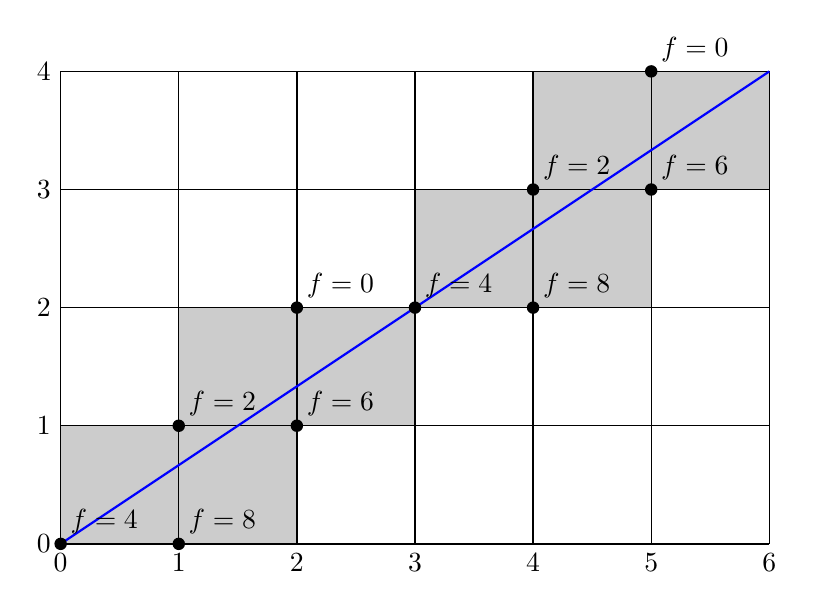
\begin{tikzpicture}[scale=1.5,line width=0.5pt]
    \draw (0,0) grid (6,4);

    \node[below] at (0,0) {0};
    \node[below] at (1,0) {1};
    \node[below] at (2,0) {2};
    \node[below] at (3,0) {3};
    \node[below] at (4,0) {4};
    \node[below] at (5,0) {5};
    \node[below] at (6,0) {6};

    \node[left] at (0,0) {0};
    \node[left] at (0,1) {1};
    \node[left] at (0,2) {2};
    \node[left] at (0,3) {3};
    \node[left] at (0,4) {4};

    \filldraw[color=black,fill=black!20] (0,0) rectangle (1,1); 
    \filldraw[color=black,fill=black!20] (1,0) rectangle (2,1);
    \filldraw[color=black,fill=black!20] (1,1) rectangle (2,2);
    \filldraw[color=black,fill=black!20] (2,1) rectangle (3,2);
    \filldraw[color=black,fill=black!20] (3,2) rectangle (4,3); 
    \filldraw[color=black,fill=black!20] (4,2) rectangle (5,3);
    \filldraw[color=black,fill=black!20] (4,3) rectangle (5,4);
    \filldraw[color=black,fill=black!20] (5,3) rectangle (6,4);
    
    \draw[blue, thick] (0,0) -- (6,4);
  
    \node[above right] at (0,0) {$f=4$}; \fill (0,0) circle (1.5pt);
    \node[above right] at (1,0) {$f=8$}; \fill (1,0) circle (1.5pt);
    \node[above right] at (1,1) {$f=2$}; \fill (1,1) circle (1.5pt);
    \node[above right] at (2,1) {$f=6$}; \fill (2,1) circle (1.5pt);
    \node[above right] at (2,2) {$f=0$}; \fill (2,2) circle (1.5pt);
    \node[above right] at (3,2) {$f=4$}; \fill (3,2) circle (1.5pt);
    \node[above right] at (4,2) {$f=8$}; \fill (4,2) circle (1.5pt);
    \node[above right] at (4,3) {$f=2$}; \fill (4,3) circle (1.5pt);
    \node[above right] at (5,3) {$f=6$}; \fill (5,3) circle (1.5pt);
    \node[above right] at (5,4) {$f=0$}; \fill (5,4) circle (1.5pt);

  \end{tikzpicture}
  \caption{Line of sight algorithm} \label{fig:lineofsight}
\end{figure}

\begin{algorithm}[htp]
  \SetAlgoLined\DontPrintSemicolon
  \SetKwFunction{los}{LineOfSight}
  \SetKwProg{myDef}{def}{}{}
  \myDef{\los($n_{source}$,$n_{goal}$)}{
    \nl $ x \gets n_{source}.x$\;
    \nl $ y \gets n_{source}.y$\;
    \nl $ x_{goal} \gets n_{goal}.x$\;
    \nl $ y_{goal} \gets n_{goal}.y$\;
    \nl $ dx \gets x_{goal} - x$\;
    \nl $ dy \gets y_{goal} - y$\;
    \nl $ f \gets 0$\;
    \nl \While{$x \neq x_{goal}$} {
      \nl $f \gets f + dy$\;
      \nl \uIf{$x \geq dx$} {
        \nl \uIf{$cell_{x,y}.isBlocked()$} {
          \nl \KwRet{$false$}\;
        }
        \nl $y \gets y+1$\;
        \nl $f \gets f - 1$\;
      }
      \nl \uIf{$f \neq 0 \land cell_{x,y}.isBlocked()$} {
        \nl \KwRet{$false$}\;
      }
      \nl \uIf{$dy = 0 \land cell_{x,y}.isBlocked() \land cell_{x,y-1}.isBlocked()$} {
        \nl \KwRet{$false$}\;
      }
      \nl $x \gets x + 1$\;
    }
    \nl \KwRet{$true$}\;
  }
  \caption{{\sc LineOfSight}}
\end{algorithm} 

\subsection{Algorithm Data}

Each {\tt MapInstance} has a {\tt Map}, a {\tt Graph} and an {\tt AlgorithmData} object for each of the algorithms that have been run on that map.\\

\begin{figure}
\centering
\begin{tikzpicture} [scale=1.2]
\umlsimpleclass{MapInstance} 
\umlsimpleclass[x=-4,y=-2.5]{Map} 
\umlsimpleclass[x=0,y=-2.5]{Graph}
\umlsimpleclass[x=4,y=-2.5,type=abstract]{AlgorithmData}
\umlsimpleclass[x=-4,y=-5]{Cell} 
\umlsimpleclass[x=0,y=-5]{Node} 
%\umlclass[x=4,y=-3,type=abstract]{AlgorithmData}{- distance : $double$ \\ - angle : $double$ \\ - path : $List<Coordinate>$ \\ ...}{+ go() : void \\ \# getPath($graph : Graph$) : $Node$ \\ ...} 
\umlHVuniassoc[arg1=1, pos1=0.2, align1=left,arg2=1, pos2=2, align2=right]{MapInstance}{Map}
\umluniassoc[arg1=1, pos1=0.3, align1=right,arg2=1, pos2=1, align2=right]{MapInstance}{Graph}
\umlHVuniassoc[arg1=1, pos1=0.2, align1=right, arg2=6, pos2=2, align2=right]{MapInstance}{AlgorithmData}
\umluniassoc[arg1=1, pos1=0.3, align1=right,arg2=*, pos2=1, align2=right]{Map}{Cell}
\umluniassoc[arg1=1, pos1=0.3, align1=right,arg2=*, pos2=1, align2=right]{Graph}{Node}
\umluniassoc[mult1=1,pos1=0,mult2=*,pos2=1, angle1=-45, angle2=-135, loopsize=3cm]{Node}{Node}
\end{tikzpicture}
\caption{Composition of {\tt MapInstance}}
\end{figure}

\noindent
{\tt AlgorithmData} is an abstract class to facilitate adding new algorithms in a modular way. It has a public method {\tt go()}, as well as getter methods for all statistical data about each algorithm. {\tt go()} calls the $getPath(n_{start},n_{goal})$ method, which returns $n_{goal}$ if a path is found, or $null$ otherwise. If $null$ is returned, this is recorded in the statistics. If $n_{goal}$ is returned, {\tt go()} calculates some of the statistics as follows:

\begin{description}
\item {\bf Path length}\\ \hfill
the sum of the Euclidean distances between each pair of consecutive nodes in the path.
\item {\bf Cumulative path angle}\\ \hfill
the sum of the scalar product between each pair of adjacent path segments in the path.
\item {\bf Graph calculation time}\\ \hfill
{\tt System.nanoTime()} is used to calculate the duration between the call to {\tt generateGraph()} and it returning.
\item {\bf Path calculation time}\\ \hfill
{\tt System.nanoTime()} is used to calculate the duration between the call to {\tt getPath()} and it returning.
\item {\bf Number of nodes expanded}\\ \hfill
a counter was incremented each time a node was expanded. It should be noted that in Block A*, node expansion is not the same as block expansion.
\end{description}

\section{Algorithms}

To emphasise the close relationships between the algorithms and allow for maximum code re-use, I organised the concrete instances of {\tt AlgorithmData} in a hierarchy. This also ensured that any performance differences between algorithms was due to the different nature of each algorithm and not different implementation of similar concepts. See Figure 3.5.\\

\begin{figure}
\centering
\begin{tikzpicture} [scale=1]
\umlemptyclass[type=abstract]{AlgorithmData}
\umlemptyclass[x=-2,y=-3]{Dijkstra}
\umlemptyclass[x=2,y=-3]{BlockAStar}
\umlemptyclass[x=-2,y=-6]{AStar}
\umlemptyclass[x=-2,y=-9]{AStarSmoothed}
\umlemptyclass[x=2,y=-9]{ThetaStar}
\umlemptyclass[x=2,y=-12]{LazyThetaStar}
\umlVHVreal{Dijkstra}{AlgorithmData}
\umlVHVreal{BlockAStar}{AlgorithmData}
\umlVHVinherit{AStar}{Dijkstra}
\umlVHVinherit{AStarSmoothed}{AStar}
\umlVHVinherit{ThetaStar}{AStar}
\umlVHVinherit{LazyThetaStar}{ThetaStar}

\end{tikzpicture}
\caption{Inheritance structure of algorithms}
\end{figure}

\subsection{Dijkstra's shortest paths}

The implementation was based on the pseudo-code seen in section 2.2.1. Details of note include:
\begin{description}
  \item {\bf Open Set}\\ \hfill
  the standard {\tt java.util.PriorityQueue} would occasionally not return the node with the smallest g-value when $openSet.pop()$ was called. This is a documented bug for large queues that occurs when a queue item has its priority\footnote{In this case, the {\tt Node}'s g-value} altered while residing in the $openSet$, so l had to manually $pop()$, $update()$ and re-$add()$ any node that needed to be updated when already in the $openSet$.
  \item {\bf Closed set}\\ \hfill
  the only two operations on the {\tt closedSet} are adding and checking for membership. Therefore, a {\tt HashSet} was used for its average case O(1) insertion and search speed.
  \item {\bf Extensibility} \\ \hfill
  to allow a clear algorithm hierarchy, I needed to add a call to $initialise(n)$ whenever a node $n$ was popped from the $openSet$, and a $postProcessing(n)$ step before the node is returned. In {\tt Dijkstra} these have empty method bodies, but some of the algorithms that inherit from Dijkstra will override these methods.
  \end{description}


\subsection{A*}

The implementation was based on the pseudo-code seen in section 2.2.2: A* inherits from Dijkstra, and overrides the $updateCost()$ function.

\subsection{A* with post-smoothing}

The implementation was based on the pseudo-code seen in section 2.2.3: A* inherits from A* with post-smoothing and implements its post-smoothing by overriding the $postProcessing()$ function.\\

\subsection {Basic $\theta ^{*}$ and Lazy $\theta ^{*}$}

The implementation was based on the pseudo-code seen in section 2.2.4 and 2.2.5: 
\begin{description}
\item{\bf Basic $\theta ^{*}$}\\ \hfill inherits from A*, and overrides the $updateCost()$ function
\item {\bf Lazy $\theta ^{*}$ }\\ \hfill inherits from Basic $\theta ^{*}$, and overrides the $initialiseNode()$ and $updateCost()$ functions
\end{description}

\subsection {Block A*}

{\bf Local Distance Database}\\

\noindent
The first challenge was to obtain an LDDB. Since there was no publicly available library containing the LDDBs, I had to create my own. Although it would have been possible to create the entries manually for the LDDB for block sizes of $2 \times 2$ cells, this would certainly not have been feasible for block sizes that were any larger, since for blocks of size {$n \times n$}, there will be $2^{n^{2}}$ possible blocks, each with $4.n.4.(n-1)$ pairs of ingress and egress coordinates, which gives over 12 million calculations for a block size of $4 \times 4$.\\

\noindent
I calculated the shortest paths using A* over visibility graphs, which gives provably optimal paths.\\

\noindent
For a given block size , I required:\\
\indent for every possible block of size {$n \times n$}\\
\indent \indent for every possible ingress-egress coordinate pair\\
\indent \indent \indent (a) the shortest path between that pair\\
\indent \indent \indent (b) a list containing every intermediate coordinate on that path.\\

\noindent
It was necessary to put these entries into a database structure that would be compact in memory and fast to load and query. Since these constraints were fundamental to the operation of the algorithm, any library or 3$^{rd}$ party database implementation could not be guaranteed to be sufficiently specialised for the task, so I implemented my own database using arrays and hash tables to ensure optimal performance and minimum space wastage.\\

\noindent
All queries to the database would need to identify a block and pair of coordinates as an input, and would receive either the length of the shortest path between those nodes, or a list of the intermediate nodes on the shortest path between those two nodes. I devised a simple bitwise encoding scheme to represent blocks as integers that would be much more space and time efficient than storing {\tt Map} objects in the database to use as comparison: each cell in the block is represented by a bit in the integer, and that bit is set if the corresponding cell is blocked. The 32 bits of the integer are sufficient for all the block sizes that are worth considering: $2 \times 2$ to $4 \times 4$.\footnotemark[1]\\

\noindent
Using this scheme, the underlying implementation of my database was an array of {\tt  HashMaps} - one {\tt HashMap} per block, with the array indexed by the code of the block. The {\tt HashMap} mapped a key: a {\tt Pair} of ingress-egress {\tt Coordinate}s, to a value: a {\tt Pair} consisting of the length (as a {\tt double}) of the shortest path and an {\tt ArrayList} of the {\tt Coordinate}s on the path.\\

\begin{figure}
    \centering
    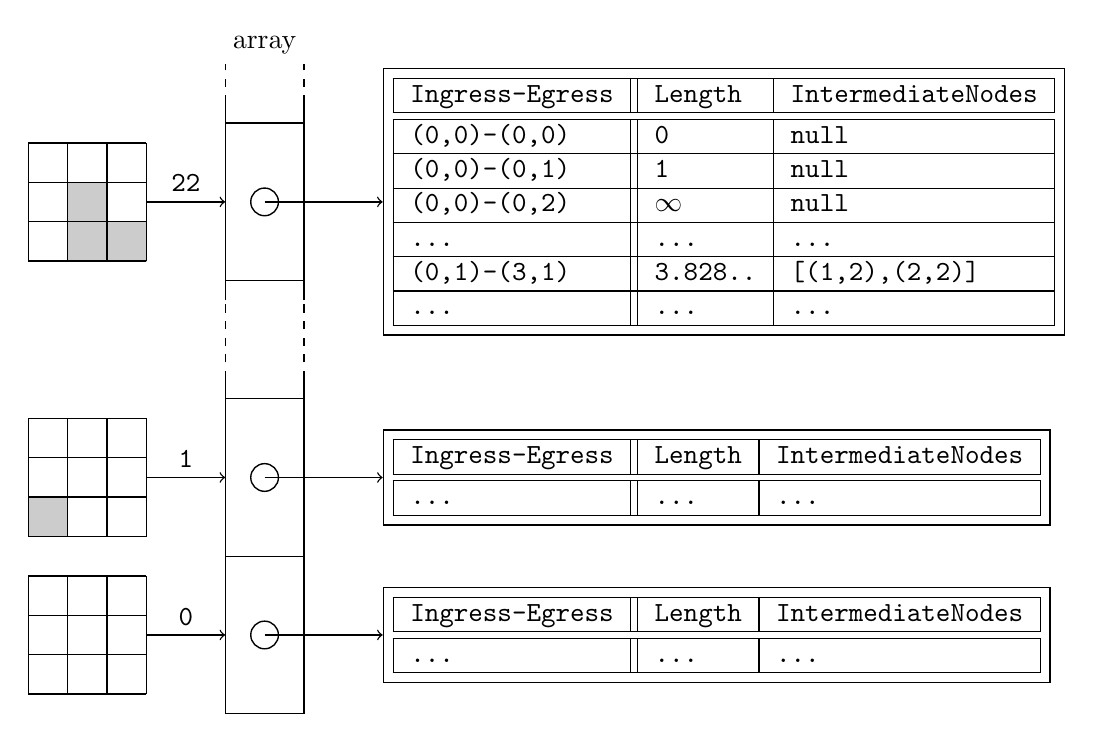
\begin{tikzpicture}[scale=0.5,line width=0.5pt]
    
    \filldraw[black!20] (0,4) rectangle (1,5);
    
    \filldraw[black!20] (1,11) rectangle (2,13);
    \filldraw[black!20] (2,11) rectangle (3,12);
    
      \draw (0,0) grid (3,3);
      \draw (0,4) grid (3,7);
      \draw (0,11) grid (3,14);
      
      \draw (5,-0.5) -- (5,8);
      \draw[dashed] (5,8) -- (5,10);
      \draw(5,10) -- (5,15);
      \draw[dashed] (5,15) -- (5,16);
      \draw (7,-0.5) -- (7,8);
      \draw[dashed] (7,8) -- (7,10);
      \draw(7,10) -- (7,15);
      \draw[dashed] (7,15) -- (7,16);
      
      \draw (5,-0.5) -- (7,-0.5);
      \draw (5,3.5) -- (7,3.5);
      \draw (5,7.5) -- (7,7.5);
      \draw (5,10.5) -- (7,10.5);
      \draw (5,14.5) -- (7,14.5);
      
      \draw[->] (3,1.5) -- (5,1.5);
      \draw[->] (3,5.5) -- (5,5.5);
      \draw[->] (3,12.5) -- (5,12.5);
      
      \node[above] at (4,1.5) {\tt 0};
      \node[above] at (4,5.5) {\tt 1};
      \node[above] at (4,12.5) {\tt 22};
      \node[above] at (6,16) {array};
      
      \draw[->] (6,1.5) -- (9,1.5);   
      \draw (6,1.5) circle (10pt);
      \node[right,draw=black,shape=rectangle] at (9,1.5) (1) {
      \begin{tabular}{| l || l | l |}
    \hline
    {\tt Ingress-Egress} & {\tt Length} & {\tt IntermediateNodes}  \\ \hline \hline
    {\tt ...}  & {\tt ...} & {\tt ...} \\ \hline
    \end{tabular}};
      \draw[->] (6,5.5) -- (9,5.5);
      \draw (6,5.5) circle (10pt);
      \node[right,draw=black,shape=rectangle] at (9,5.5) (1) {
            \begin{tabular}{| l || l | l |}
    \hline
    {\tt Ingress-Egress} & {\tt Length} & {\tt IntermediateNodes}  \\ \hline \hline
    {\tt ...}  & {\tt ...} & {\tt ...} \\ \hline
    \end{tabular}};
      \draw[->] (6,12.5) -- (9,12.5);
      \draw (6,12.5) circle (10pt);
      \node[right,draw=black,shape=rectangle] at (9,12.5) (1) {
    \begin{tabular}{| l || l | l |}
    \hline
    {\tt Ingress-Egress} & {\tt Length} & {\tt IntermediateNodes}  \\ \hline \hline
    {\tt (0,0)-(0,0)}  & {\tt 0} & {\tt null} \\ \hline
    {\tt (0,0)-(0,1)}  & {\tt 1} & {\tt null} \\ \hline
    {\tt (0,0)-(0,2)}  & {\tt $\infty$} & {\tt null} \\ \hline
    {\tt ...}  & {\tt ...} & {\tt ...} \\ \hline
    {\tt (0,1)-(3,1)}  & {\tt 3.828..} & {\tt [(1,2),(2,2)]} \\ \hline
    {\tt ...}  & {\tt ...} & {\tt ...} \\ \hline
\end{tabular}};
      

    \end{tikzpicture}
  \caption[Extract of the LDDB for block size of $3 \times 3$]{Extract of the LDDB for block size of $3 \times 3$ - array of {\tt HashTable<PairOfCoords,Pair<double,List<Coord>>}s}
  %\label{fig:fig}
\end{figure}

\noindent
This implementation was sufficient but unsatisfactory, as the database sizes were unnecessarily large. This would cause slow loading to memory, less of the LDDB stored in cache and more likelihood of thrashing. Therefore, I compressed the database using bitwise encoding schemes:
\begin{itemize}
\item each {\tt Pair} of ingress-egress {\tt Coordinate}s can be represented with a unique integer representable in a {\tt byte}'s worth of space - so a coding scheme was devised to create an efficient hash function for the {\tt PairOfCoordinate} class.
\item the {\tt List} of intermediate {\tt Coordinate}s can be represented by a code that fits into the 32 bits of an integer: since the maximum number of intermediate nodes on a shortest path in a sub map of size up to {$4 \times 4$} is four\footnotemark[2], and the range of $x$ and $y$ in the {\tt Coordinate} is 0-4, therefore 6 bits can be used for each {\tt Coordinate} - 3 for $x$, 3 for $y$, which is a maximum total of 24 bits.
\end{itemize}

\begin{figure}
\begin{lstlisting}
PairOfCoords(Coordinate c1, Coordinate c2, int blockSize) {
		this.blockSize = blockSize;
		this.coordCode = (byte) 
			(c1.getX() + 
			c1.getY() * (blockSize+1) + 
			c2.getX() * (blockSize+1)*(blockSize+1) + 
			c2.getY() * (blockSize+1)*(blockSize+1)*(blockSize+1));
	}
\end{lstlisting}
\caption{Encoding scheme for {\tt PairOfCoords} in the compressed LDDB}
\end{figure}

\begin{figure}
\begin{lstlisting}
int getListCode(List<Coordinate> intermediateNodes) {
		int listCode = 0;
		for(Coordinate c : intermediateNodes) {
			listCode = listCode | c.getX();
			listCode = listCode << 3;
			listCode = listCode | c.getY();
			listCode = listCode << 3;
		}
		listCode = listCode >>> 3;	//undoes line 7 on final loop
		return listCode;
	}
\end{lstlisting}
\caption{Encoding scheme for {\tt List<Coordinate>} in the compressed LDDB}
\end{figure}

\noindent
These compression techniques allowed me to reduce the size of the databases by about 50\%:

\begin{center}
    \begin{tabular}{| l | l | l |}
    \hline
    Submap size & Size of uncompressed LDDB & Size of compressed LDDB\footnotemark[3]$^{,}$\footnotemark[4]  \\ \hline
    {$2 \times 2$}  & 33KB  & 17KB \\ \hline
    {$3 \times 3$}  & 2.2MB & 1.1MB \\ \hline
    {$4 \times 4$}  & 485MB & 192MB \\ \hline
  \end{tabular}
\end{center}

\noindent
I will investigate the performance of the uncompressed and compressed LDDBs in the Evaluation section.\\
\\

\footnotetext[1]{The exponential increase in size of LDDB would mean that the LDDB for block sizes of $5 \times 5$ or larger take so long to search that performance benefit diminishes.}
\footnotetext[2]{Obtained by experimental results.}
\footnotetext[3]{These savings could be improved further for sub maps of size {$2 \times 2$} and {$3 \times 3$} by using specific data-types depending on the submap size, but this was unnecessary, as the LDDB size was very small compared to the total available memory for sub maps of size{$2 \times 2$} and {$3 \times 3$}, and the LDDB only needs to be loaded into memory once per run of the program.}
\footnotetext[4]{These sizes were significantly larger than those found in Yap's paper, but his agents were only allowed to travel horizontally and vertically, so only 4 bits were needed to store the path length value.}

\noindent
{\bf Special case blocks: $block_{start}$ and $block_{goal}$} \\

\noindent
$block_{start}$ and $block_{goal}$ are treated as special cases by Block A*. On initialisation:
\begin{itemize}
\item the {\em g-values} of the boundary nodes of $block_{start}$ are set by manually computing shortest paths from $n_{start}$ to each boundary node, instead of looking them up in the LDDB as with other blocks. This is because $n_{start}$ is not guaranteed to be on the boundary of a block, and the LDDB only holds details for routes between boundary nodes
\item the {\em h-values} of the boundary nodes of $block_{goal}$ are set manually for similar reasons.
\item a check is made as to whether $n_{start}$ and $n_{goal}$ are in the same block - i.e. $block_{start}$ equals $block_{goal}$. If so, the shortest path between the two is computed  manually.
\end{itemize}

\noindent
To compute these values, I created a visibility graph for the relevant block and computed the shortest path to each boundary node. Having run some preliminary tests, it became clear that on small maps these initialisations took up to 50\% of the run-time of the algorithm [insert some statistics of test runs]. Therefore, I decided to implement two alternative, extended forms of the LDDB:
\begin{description}
\item{\bf Semi-extended} contains details of shortest paths from {\em any} node to {\em any boundary} node in a block.
\item{\bf Fully-extended} contains details of shortest paths from {\em any} node to {\em any} node in a block.
\end{description}

\noindent
The increase in the size of the LDDB in comparison to the original is:
\begin{center}
    \begin{tabular}{| l | l | l |}
    \hline
    Submap size & Semi-extended & Fully-extended  \\ \hline
    {$2 \times 2$}  & 12.5\% & 26.5\% \\ \hline
    {$3 \times 3$}  & 33.3\% & 77.8\%\\ \hline
    {$4 \times 4$}  & 56.3\% & 144.1\% \\ \hline
  \end{tabular}
\end{center}

\noindent
The use of the fully-extended LDDB allows the initialisation of $block_{start}$ and $block_{goal}$ and the $block_{start}$ equals $block_{goal}$ case to use the LDDB, whereas using semi-extended LDDB requires that the $block_{start}$ equals $block_{goal}$ case finds the shortest route manually.\footnotemark[1] The performance benefits of these different forms of the LDDB will be investigated in the Evaluation chapter.\\

\footnotetext[1]{Note that when using the semi-extended LDDB, $block_{goal}$ needs to reverse the ingress-egress coordinates before querying the LDDB.}

\noindent
{\bf Block A* - algorithm} \\

\noindent
The core of the algorithm was a straightforward implementation, once the details of it were understood. The most challenging part of the implementation was the traceback stage, which was unspecified in the paper. The traceback stage extracts the coordinates of the path from the Graph structure. This requires finding and inserting into a list:
\begin{itemize}
\item the optimal path from $n_{goal}$ to the optimal ingress node of $block_{goal}$
\item the nodes on the optimal path that share block boundaries
\item the intermediate nodes where the optimal path traverses a block
\item the optimal route from the optimal egress node of $block_{start}$ to $n_{start}$
\end{itemize}
\noindent
whilst omitting from the list:
\begin{itemize}
\item all but one of any nodes in this path that lie in the same physical location but belong to different blocks: this occurs when the path crosses block boundaries.
\end{itemize}
 
\section{User Interface}

The user interface was built using Java's Swing toolkit. The UI allows the user to:
\begin{description}
\item{\bf Generate a map} of a given resolution, coverage percentage and clustering.
\item{\bf Create a map} of a given resolution using an interactive editor that has brushes and erasers of differing sizes. If the UI is in map creation mode then UI uses {\tt MouseListener}s to detect when the mouse is being dragged over the map. The array that represents the map is updated according to the size of the brush and the resolution of the map, and then the {\tt repaint()} method of the {\tt JPanel} is called. Once the creation is complete, the array is passed as a parameter to a {\tt Map} constructor, and the {\tt Map} object is passed to the Simulator.
\item{\bf Save a map} with or without paths and statistics.
\item{\bf Load a map} with or without paths and statistics.
\item{\bf Choose start and end points} for the paths on the current map. If the UI is not in map creation mode then {\tt MouseListener}s are used to detect where on the screen the mouse is clicked. The start and end points can be set anywhere on the map.
\item{\bf Calculate paths} for each of the 6 algorithms on the current map. If there is no path then {\tt NoPath} will be displayed.
\item{\bf Display paths} once the path has been calculated
\end{description}

\begin{figure}
\centering
\shadowpicture{\includegraphics[width=0.8\textwidth]{creationmode.png}}
\caption{User interface in map creation mode}
\end{figure}

\begin{figure}
\centering
\shadowpicture{\includegraphics[width=0.8\textwidth]{paths.png}}
\caption{User interface displaying paths for a generated map}
\end{figure}

\section{Testing}

\todo{Implementation: testing \ldots}

\section{Data extraction}

To harvest enough data to do meaningful statistical analysis of the performance of the algorithms, the simulator was designed to have a simple API that allowed both a UI to be bolted on and scripts that could bypass the UI altogether. I used the open source package {\tt CSVWriter} to write the data obtained to CSV files, as these are the standard input for $R$ based statistical analysis.

\begin{figure}
\centering
    \begin{tabular}{| l | l | l | l | l |}
    \hline
    Map & Algorithm & PathTime & TotalLength & TotalAngle\\ \hline % & NodesExp\\ \hline
     Map 1 & Dijkstra & 852.926976 & 160.752308679 & 495.0000736525\\ \hline % & 8203\\ \hline
     Map 1 & AStar & 169.831936 & 160.752308679 & 855.0000688228\\ \hline %  & 2999\\ \hline
     Map 1 & AStarVisibility & 5.334016 & 151.6768359881 & 102.262577962\\ \hline %  & 289\\ \hline
Map 1 & AStarSmoothed & 85.908992 & 154.9127142045 & 165.3889464848\\ \hline %  & 2999\\ \hline
Map 1 & ThetaStar & 30.230016 & 151.7637935619 & 122.1222152092\\ \hline %  & 1682\\ \hline
Map 1 & LazyThetaStar & 32.45824 & 151.7637935619 & 122.1222152092\\ \hline %  & 1692\\ \hline
Map 1 & BlockAStar & 10.85792 & 152.8713149055 & 566.7296353554\\ \hline %  & 3278\\ \hline
Map 2 & Dijkstra & 615.220992 & 161.3380951166 & 810.0000676154\\ \hline %  & 8146\\ \hline
 \end{tabular}
\caption{Extract from a CSV file exported by {\tt DataExtract}}
\end{figure}

\begin{figure}
\begin{lstlisting}
void generateMaps 
	(int size, int coverage, int clustering, int numberOfMaps) {
	
	for(int i=0;i<numberOfMaps;i++) {
		saveMapOnly(size+"/"+coverage+"/"+clustering+"/"+i+".ser",
			new MapInstance(
				MapGenerator.generateMap(size,size,coverage,clustering)));
	}
}
\end{lstlisting}
\caption{Code snippet from {\tt DataExtraction} showing automation of {\tt Graph} creation}
\end{figure}

\begin{figure}
    \centering
    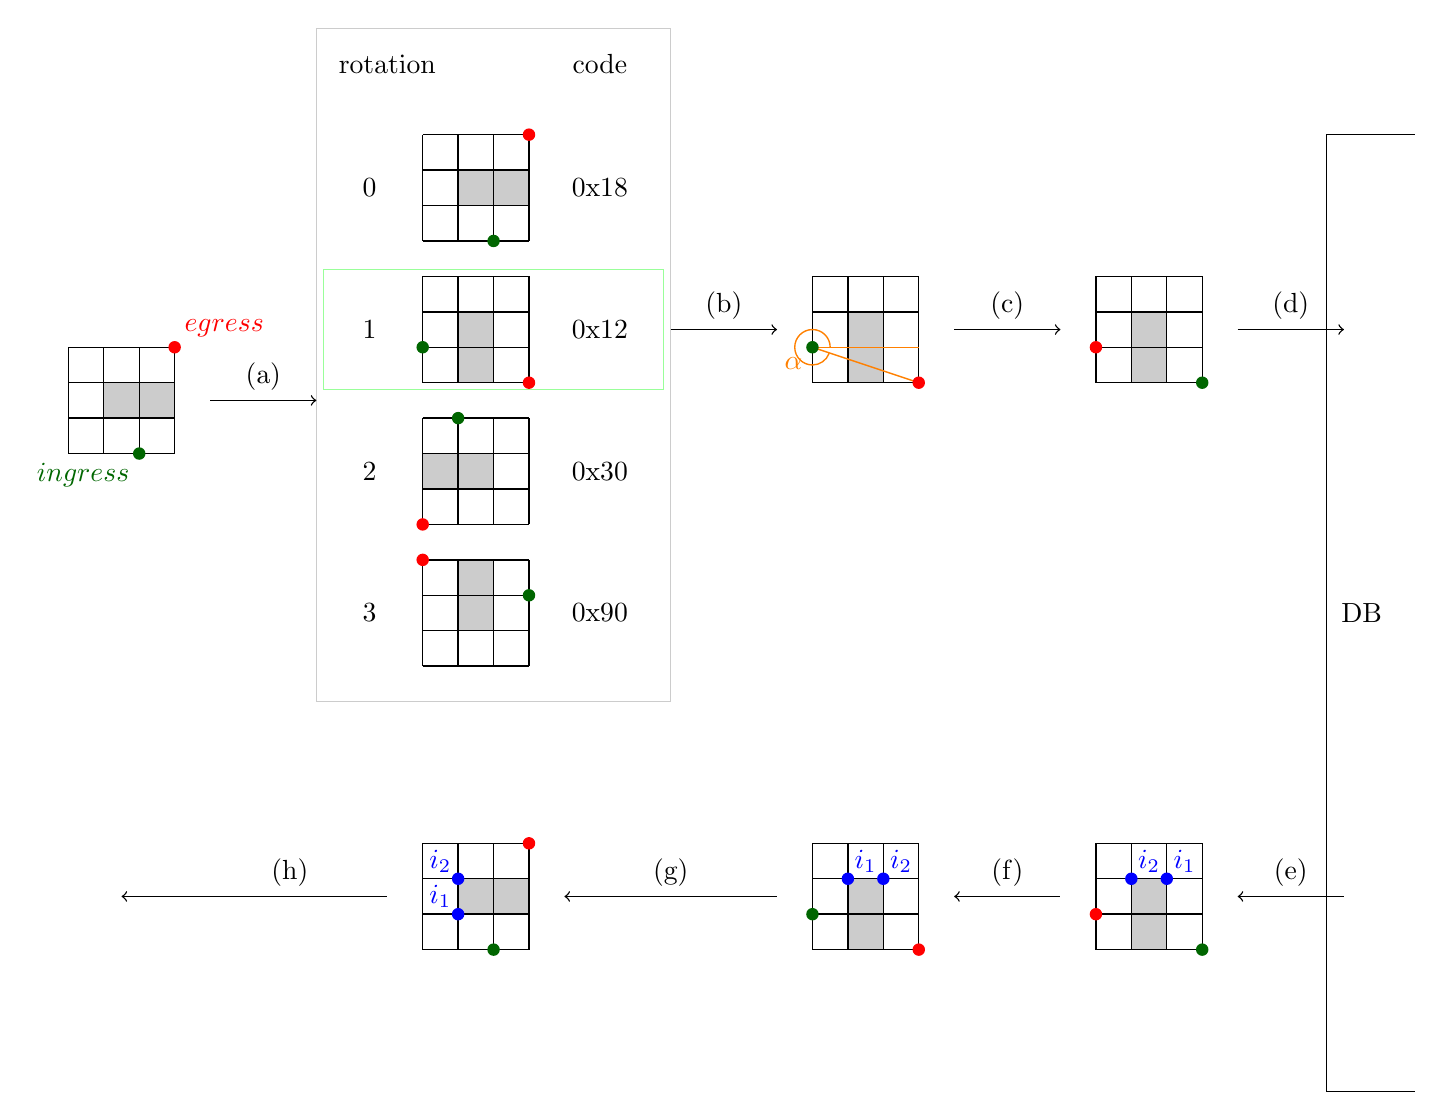
\begin{tikzpicture}[scale=0.45,line width=0.5pt]
    
    %input
    \filldraw[black!20] (-9,7) rectangle (-7,8);
    \draw (-10,6) grid (-7,9);
    \fill[black!60!green] (-8,6) circle (5pt);
    \node[below left, black!60!green] at (-8,6) {$ingress$};
    \fill[red] (-7,9) circle (5pt);
    \node[above right, red] at (-7,9) {$egress$};
    
    %rotations
    \draw[black!20] (-3,-1) rectangle (7,18);
    \draw[green!40] (-2.8,7.8) rectangle (6.8,11.2);
    
    \filldraw[black!20] (1,13) rectangle (3,14);
    \draw (0,12) grid (3,15);
    \fill[black!60!green] (2,12) circle (5pt);
    \fill[red] (3,15) circle (5pt);
        
    \filldraw[black!20] (1,8) rectangle (2,10);
    \draw (0,8) grid (3,11);
    \fill[black!60!green] (0,9) circle (5pt);
    \fill[red] (3,8) circle (5pt);
        
    \filldraw[black!20] (0,5) rectangle (2,6);
    \draw (0,4) grid (3,7);
    \fill[black!60!green] (1,7) circle (5pt);
    \fill[red] (0,4) circle (5pt);
    
    \filldraw[black!20] (1,1) rectangle (2,3);
    \draw (0,0) grid (3,3);
    \fill[black!60!green] (3,2) circle (5pt);
    \fill[red] (0,3) circle (5pt);
    
    \draw[->] (-6,7.5) -- (-3,7.5);
    \node[above] at (-4.5,7.5) {(a)};
    
    \node at (-1,17) {rotation};	\node at (5,17) {code};
    \node at (-1.5,13.5) {0};		\node at (5,13.5) {0x18};
    \node at (-1.5,9.5) {1};		\node at (5,9.5) {0x12};
    \node at (-1.5,5.5) {2};		\node at (5,5.5) {0x30};
    \node at (-1.5,1.5) {3};		\node at (5,1.5) {0x90};
    
    \draw[->] (7,9.5) -- (10,9.5);
    \node[above] at (8.5,9.5) {(b)};
   
   %angle check
    \filldraw[black!20] (12,8) rectangle (13,10);
    \draw (11,8) grid (14,11);
    \draw[orange] (11,9) -- (14,9);
    \draw[orange] (11,9) -- (14,8);
    \draw[orange] (11.5,9) arc (0:340:0.5);
    \node[below left, orange] at (11,9) {$\alpha$};
    \fill[black!60!green] (11,9) circle (5pt);
    \fill[red] (14,8) circle (5pt);
    
    \draw[->] (15,9.5) -- (18,9.5);
    \node[above] at (16.5,9.5) {(c)};
    
    %DB input
    \filldraw[black!20] (20,8) rectangle (21,10);
    \draw (19,8) grid (22,11);
    \fill[red] (19,9) circle (5pt);
    \fill[black!60!green] (22,8) circle (5pt);
    
    \draw[->] (23,9.5) -- (26,9.5);
    \node[above] at (24.5,9.5) {(d)};
    \draw (25.5,15) -- (28,15);
    \draw (25.5,-12) -- (28,-12);
    \draw (25.5,-12) -- (25.5,15);
    \node at (26.5,1.5) {DB};
        
    \draw[<-] (23,-6.5) -- (26,-6.5);
    \node[above] at (24.5,-6.5) {(e)};
    
    %DB output
    \filldraw[black!20] (20,-8) rectangle (21,-6);
    \draw (19,-8) grid (22,-5);
    \fill[red] (19,-7) circle (5pt);
    \fill[black!60!green] (22,-8) circle (5pt);
    \fill[blue] (21,-6) circle (5pt);
    \node[blue] at (21.5,-5.5) {$i_{1}$};
    \fill[blue] (20,-6) circle (5pt);
    \node[blue] at (20.5,-5.5) {$i_{2}$};
    
    \draw[<-] (15,-6.5) -- (18,-6.5);
    \node[above] at (16.5,-6.5) {(f)};
    
    %flipped
    \filldraw[black!20] (12,-8) rectangle (13,-6);
    \draw (11,-8) grid (14,-5);
    \fill[black!60!green] (11,-7) circle (5pt);
    \fill[red] (14,-8) circle (5pt);
    \fill[blue] (12,-6) circle (5pt);
    \node[blue] at (12.5,-5.5) {$i_{1}$};
    \fill[blue] (13,-6) circle (5pt);
    \node[blue] at (13.5,-5.5) {$i_{2}$};
    
    \draw[<-] (4,-6.5) -- (10,-6.5);
    \node[above] at (7,-6.5) {(g)};
    
    %rotated
    \filldraw[black!20] (1,-7) rectangle (3,-6);
    \draw (0,-8) grid (3,-5);
    \fill[black!60!green] (2,-8) circle (5pt);
    \fill[red] (3,-5) circle (5pt);
    \fill[blue] (1,-7) circle (5pt);
    \node[blue] at (0.5,-6.5) {$i_{1}$};
    \fill[blue] (1,-6) circle (5pt);
    \node[blue] at (0.5,-5.5) {$i_{2}$};
    
    \draw[<-] (-8.5,-6.5) -- (-1,-6.5);
    \node[above] at (-3.75,-6.5) {(h)};


    \end{tikzpicture}
  \caption{my caption}
  %\label{fig:fig}
\end{figure}


\chapter{Evaluation}

\chapter{Conclusion}

\bibliography{refs}{}
\bibliographystyle{unsrt}

\appendix




\cleardoublepage

\end{document}